\chapter{Autoregulon Networks: COMING SOON}
\label{ch-autoregulons}


This chapter is mostly based on Ref.\cite{alon-book},
a textbook by Uri Aron 
on {\bf Systems Biology}. That book divides its chapters into 3 \qt{Parts}: Network Motifs, Robustness and Optimality. This chapter covers only the first part, {\bf Network Motifs} (NM). {\bf Autoregulon networks}
is an alternative name for NM. 

In this chapter, we discuss,
from a causal inference perspective, a  special 
class of 
S1ODE (system of first order ordinary differential equations) that occurs in biology/genomics.
 Ref.\cite{alon-book} by Alon
 has a much broader scope. Like this chapter, 
Alon's book describes the mathematical aspects of the
 S1ODEs. But it 
also describes  in detail where they occur in biology/genomics and what experimental data exists in support
of the assertion that they are 
realized in Nature. We discuss briefly the biological
underpinnings of the math, but 
to a much lesser extent than Alon's book.
If you are new to genomics, and would like to follow that discussion, you might find Appendix \ref{ch-genomics-vocab} helpful.

I will assume
the reader has read 
 Chapter \ref{ch-dynamical-sys}
on Dynamical Systems before reading this one.



\section{Hill functions}

We  will use 2  kinds of {
\bf Hill functions}.
\begin{itemize}
\item {\bf Activator Hill function} (highpass filter)
 \beq
 h_{\oplus}(x; \beta, K, n)
 =\beta\frac{\left(\frac{x}{K}\right)^n}{1 + \left(\frac{x}{K}\right)^n}
 \eeq
 
 Note that
 
 \beq
 \begin{array}{ll}
 h_\oplus(x)
 \rarrow \beta\indi(x>K) 
 &\text{as } n\rarrow\infty
 \\
 h_\oplus(x)
 \approx
 \frac{\beta}{2}
 \left[
 1 + \frac{n}{2}\left(
 \frac{x}{K}-1
 \right)
 \right]
 &\text{for $x\approx K$}
 \end{array}
 \eeq
 
 \item {\bf Repressor  Hill function} (lowpass filter)
 
 \beq
  h_{\ominus}(x; \beta, K, n)=\beta\frac{1}{1 + \left(\frac{x}{K}\right)^n}
  \eeq
  
  Note that
  
  \beq
  \begin{array}{ll}
  h_\ominus(x; \beta, K)
  \rarrow\beta\indi(x<K) 
  &\text{ as } n\rarrow\infty
 \\
  h_\ominus(x)\approx
  \frac{\beta}{2}
  \left[
  1 -\frac{n}{2}\left(
  \frac{x}{K}-1
  \right)
  \right]
  &\text{for $x\approx K$}
  \end{array}
  \eeq
\end{itemize}

Note that
\beq
h_\oplus(x)+h_\ominus(x)=\beta
\eeq

Figs.\ref{fig-hill-n-1}, 
\ref{fig-hill-n-2} and \ref{fig-hill-n-10}
are plots of $h_\oplus(x)$ and $h_\ominus(x)$
for $n=1$, $n=2$ and $n=10$, respectively, assuming $\beta=K=1$.

The Hill functions are not
just some abstract concept
unrelated to Nature. They are
observed in Nature,
and they
can be derived using Chemistry.

\begin{figure}[h!]
\centering
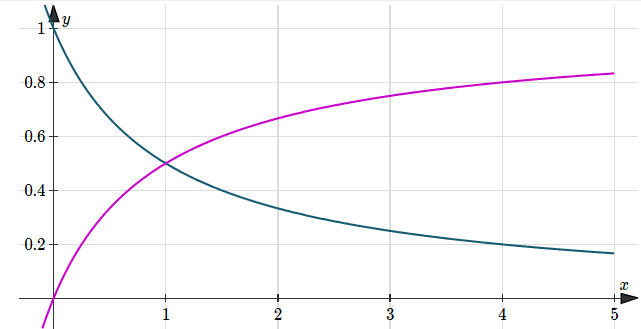
\includegraphics[width=4.3in]
{autoregulons/hill-1.png}
\caption{Plot of $y= 1/(1+x^n)$
and $y=x^n/(1+x^n)$ for $n=1$.}
\label{fig-hill-n-1}
\end{figure}

\begin{figure}[h!]
\centering
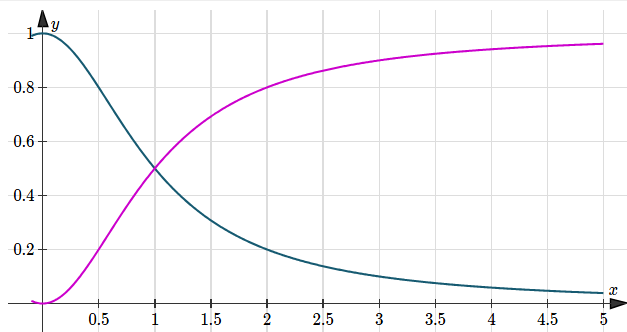
\includegraphics[width=4.3in]
{autoregulons/hill-2.png}
\caption{Plot of $y= 1/(1+x^n)$
and $y=x^n/(1+x^n)$ for $n=2$.}
\label{fig-hill-n-2}
\end{figure}

\begin{figure}[h!]
\centering
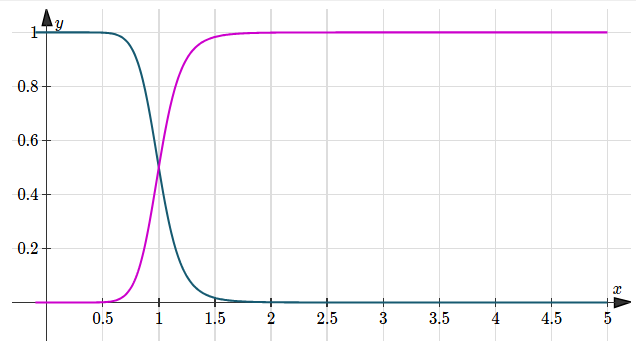
\includegraphics[width=4.3in]
{autoregulons/hill-10.png}
\caption{Plot of $y= 1/(1+x^n)$
and $y=x^n/(1+x^n)$ for $n=10$.}
\label{fig-hill-n-10}
\end{figure}

\section{One Autoregulon}

The ODEs of this chapter can be represented by bnets
in which variables like $x$ and 
their velocities (i.e., time derivatives)
like $\dot{x}$,
are nodes.
Subgraphs of such bnets, especially those
subgraphs that recur frequently as building blocks, are called
a {\bf network motifs}.  The most basic
of the network motifs is the {\bf autoregulon},
which we describe next.  All bnets
in this chapter can be viewed as {\bf autoregulon
networks}.


This is the autoregulon net motif: 

\beq
\xymatrix{
&\rvx\ar[dd]|{-\alp}\ar[dl]
\\
h(\rvx)\ar[dr]|{1}
\\
&\dot{x}
}\quad
\xymatrix{\\=}
\quad
\xymatrix{
\\
\rvx\ar@{=>}[d]
\\
\dot{\rvx}
}
\xymatrix{\\=}
\quad
\xymatrix{\\\Rect{\rvx}}
\quad
\left\{
\dot{x}=\underbrace{-\alp x + h(x)}_{f(x)}
\right.
\label{eq-1-autoreg}
\eeq
Eq.(\ref{eq-1-autoreg}) also defines  the 2 symbols
\begin{itemize}
\item double arrow pointing from a random variable and 
to its time derivative,
\item boxed random variable
\end{itemize}
that we will
use to represent a single autoregulon when we 
represent
networks of autoregulons.



Let $\alp, \beta >0$.
In general, $h(x)$ is either the $\oplus$ or $\ominus$ Hill function.
However, we often use the following approximations
\beq
h(x)=\left\{
\begin{array}{ll}
\beta\indi(x>K)
&(\text{ideal highpass filter})
\\
\beta\indi(x<K)
&(\text{ideal lowpass filter})
\\
h_0+|h_1| x
&(\text{positive feedback})
\\
h_0 -|h_1| x
&(\text{negative feedback})
\end{array}
\right.
\eeq

\subsection{Autoregulon notation}
Henceforth, we will use

\begin{itemize}
\item
$\xymatrix{\Rect{\rvx}}$ to denote any 
autoregulon $\rvx$

\item
$\xymatrix{\Rect{\rvx^\redoplus}}$ to denote a highpass 
autoregulon $\rvx$

\item
$\xymatrix{\Rect{\rvx^\redominus}}$ to denote a lowpass 
autoregulon $\rvx$

\item
$\xymatrix{\Rect{\rvx^\redplus}}$ to denote a positive feedback 
autoregulon $\rvx$


\item  $\xymatrix{\Rect{\rvx^\redminus}}$
to denote a negative feedback 
autoregulon $\rvx$. \footnote{
Ref.\cite{alon-book}
denotes a negative feedback autoregulon by 
$\xymatrix{\rvx\loopright{3}{@{-|}}}$
} 

\item $\xymatrix{\rvx\ar[r]^\alp&\rvy}$ to denote $\rvy = \alp \rvx$.

 \item  $\xymatrix{\rvx\ar[r]|\redplus&\rvy}$
to denote
$\xymatrix{\rvx\ar[r]^\alp&\rvy}
$
with $\alp>0$.

\item  $\xymatrix{\rvx\ar[r]|\redminus&\rvy}$
to denote
$\xymatrix{\rvx\ar[r]^\alp&\rvy}$
with $\alp<0$\footnote{
Ref.\cite{alon-book}
represents $\xymatrix{\rvx\ar[r]|\redminus&\rvy}$ as $\xymatrix{\rvx\ar@{-|}[r]&\rvy}$
}

\item  $\xymatrix{\rvx\ar[r]|\redzero&\rvy}$
to denote
$\xymatrix{\rvx\ar[r]^\alp&\rvy}$
with $\alp=0$.

\item  $\xymatrix{\rvx\ar[r]|\redominus^K
&\rvy}$
to denote
$h_\ominus(x)$
for some $K>0$

\item  $\xymatrix{\rvx\ar[r]|\redoplus^K
&\rvy}$
to denote
$h_\oplus(x)$
for some $K>0$

\end{itemize}

Note that 
near $x=K$, $h_{\oplus}$ is
approximately linear
with positive slope.
Hence,  $h_{\oplus}$
is closely related to positive feedback, as their symbols
$\redoplus$ and $\redplus$ suggest. 

The last paragraph is still true if we replace the terms (positive, $\redoplus$, 
$\redplus$) by 
(negative, $\redominus$, 
$\redminus$).

If an arrow in a net has no sign, assume its sign 
might be either plus or minus.

Sometimes we want to write an expression
such as $\alp x -\beta y$ for some $\alp, \beta>0$ but we don't want to specify
the names of the coefficients $\alp, \beta$.
In such cases, we will write $\PP x -\PP y$
instead of $\alp x -\beta y$. In general,
\begin{itemize}
\item
$\PP x$ means $\alp x$ for some $\alp>0$.
\item
$-\PP x$ means $\alp x$ for some $\alp<0$.
\item
$\RR x$ means $\alp x$ for some $\alp\in \RR$.
\end{itemize}

\subsection{Potential function}

Let

\beq
\dot{x} = \underbrace{-\alp x + h(x)}_{f(x)}
\eeq

\beq
h(x)= h_0 + h_1x
\eeq
Then

\beqa
f(x)
&=&h_0
-\underbrace{(\alp-h_1)}_{\alp_1} x
\\
&=&
-\alp_1(x-x_a)
\eeqa
where
$x_a = \frac{h_0}{\alp_1}$.

Recall from Chapter \ref{ch-dynamical-sys}
that


\beq
V-V_0= -\int^x dx\; f(x)=\frac{\alp_1}{2}(x-x_a)^2
\label{eq-v-for-general-linear-h}
\eeq
$V_0$ is arbitrary, but note that $V(x)$ must be continuous
because, since $\dot{x}=-\partial_xV(x)$, a jump in $V(x)$
would produce an infinity in $\dot{x}$.

\begin{figure}[h!]
\centering
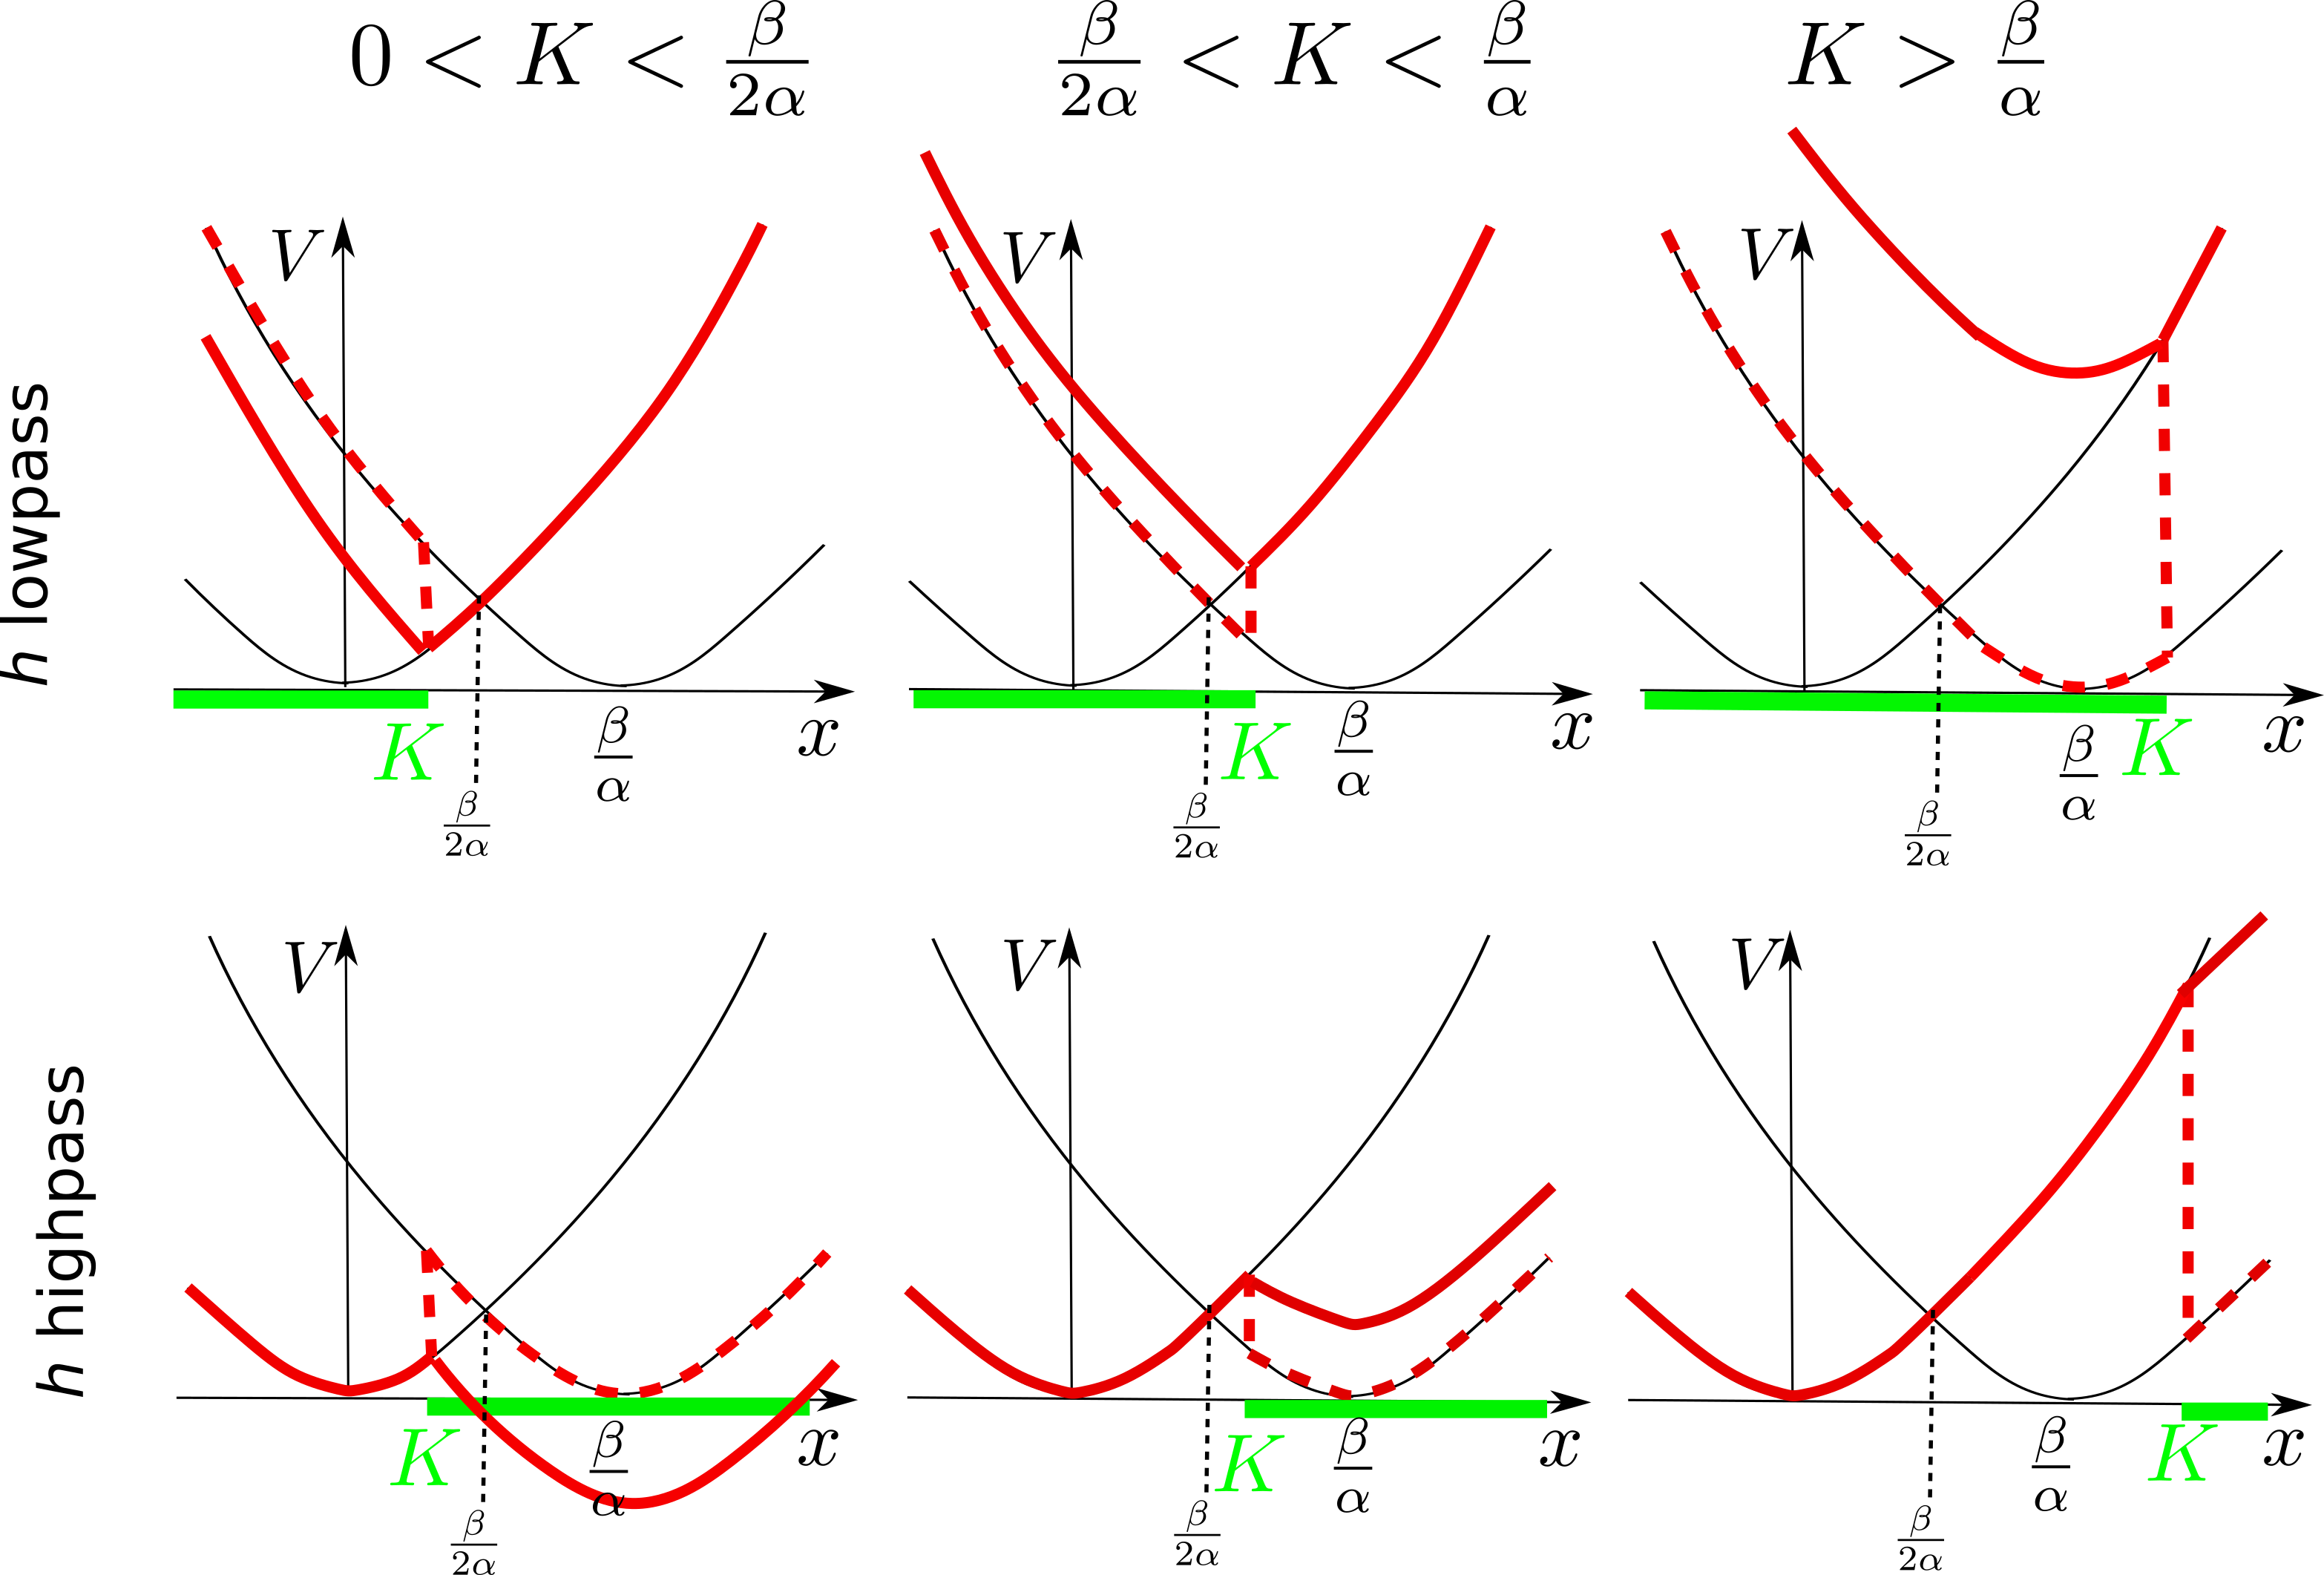
\includegraphics[width=4.7in]
{autoregulons/v-low-high-pass.png}
\caption{Highpass
and lowpass $V(x)$ (in red), for various 
ranges of $K$.
$h(x)$ is zero outside green regions of $x$ axis.
Note that when $V_0=0$, $V$ has two branches: two
parabolas with the same second derivative but different vertices. 
By symmetry, their intersection is
at $x=\frac{x_\beta}{2}$,
midway between the vertices.}
\label{fig-v-low-high-pass}
\end{figure}

Eq.(\ref{eq-v-for-general-linear-h})
for linear $h$
can be used to analyze the following
3 cases
in which $h$
is piece-wise linear:

\begin{enumerate}
\item {\bf ideal lowpass filter}

When 

\beq
h(x)=\beta\indi(x<K)
\eeq
we have

\beq
h_0 = \left\{
\begin{array}{ll}
\beta &\text{if $x<K$}
\\
0 & \text{if $x>K$}
\end{array}
\right\}
,\quad
h_1=0
\eeq
Hence,

\beq
V=
\left\{
\begin{array}{ll}
\frac{\alp}{2}(x-x_\beta)^2 + V_0
&\text{if $x<K$}
\\
\frac{\alp}{2}x^2
&\text{if $x>K$}
\end{array}
\right.
\eeq
where 
$x_\beta =\frac{\beta}{\alp}$,
and $V_0$ is defined so that $V(x)$ is the same for $x=K\pm\eps$
where $0<\eps<<0$.

See Fig.\ref{fig-v-low-high-pass} for a plot of this $V$.
From that figure,
we learn that if $h$ is lowpass, the potential has one minimum:

\begin{itemize}[$\checkmark$]
\item at $x=K$ if $K<\frac{\beta}{\alp}$,

\item at $x=\frac{\beta}{\alp}$ if $K>\frac{\beta}{\alp}$.

\end{itemize}

\item {\bf ideal highpass filter}

If 

\beq
h(x)=\beta\indi(x>K)
\eeq
then

\beq
h_0 = \left\{
\begin{array}{ll}
0 &\text{if $x<K$}
\\
\beta & \text{if $x>K$}
\end{array}
\right\},\quad
h_1=0
\eeq
Hence,

\beq
V=
\left\{
\begin{array}{ll}
\frac{\alp}{2}x^2
&\text{if $x<K$}
\\
\frac{\alp}{2}(x-x_\beta)^2 + V_0
&\text{if $x>K$}
\end{array}
\right.
\eeq
where 
$x_\beta =\frac{\beta}{\alp}$,
and $V_0$ is defined so that $V(x)$ is the same for $x=K\pm\eps$
for $0<\eps<<0$.

See Fig.\ref{fig-v-low-high-pass} for a plot of this $V$.
From that figure, we learn that if $h$ is highpass, it has one or two minima:

\begin{itemize}[$\checkmark$]
\item at $x=0$ and $x=\frac{\beta}{\alp}$ if $K<\frac{\beta}{\alp}$,

\item at $x=0$ if $K>\frac{\beta}{\alp}$

\end{itemize}


\item {\bf linear $h$} (positive feedback if $h_1>0$,
negative feedback otherwise)

When

\beq
h(x)\approx h_0 + h_1x
\eeq
we have

\beq
V= \frac{\alp_1}{2}(x-x_a)^2
\eeq

See Fig.\ref{fig-v-low-high-pass}
for a plot of this $V$ for various 
choices of $\alp_1=\alp-h_1$.

\begin{figure}[h!]
\centering
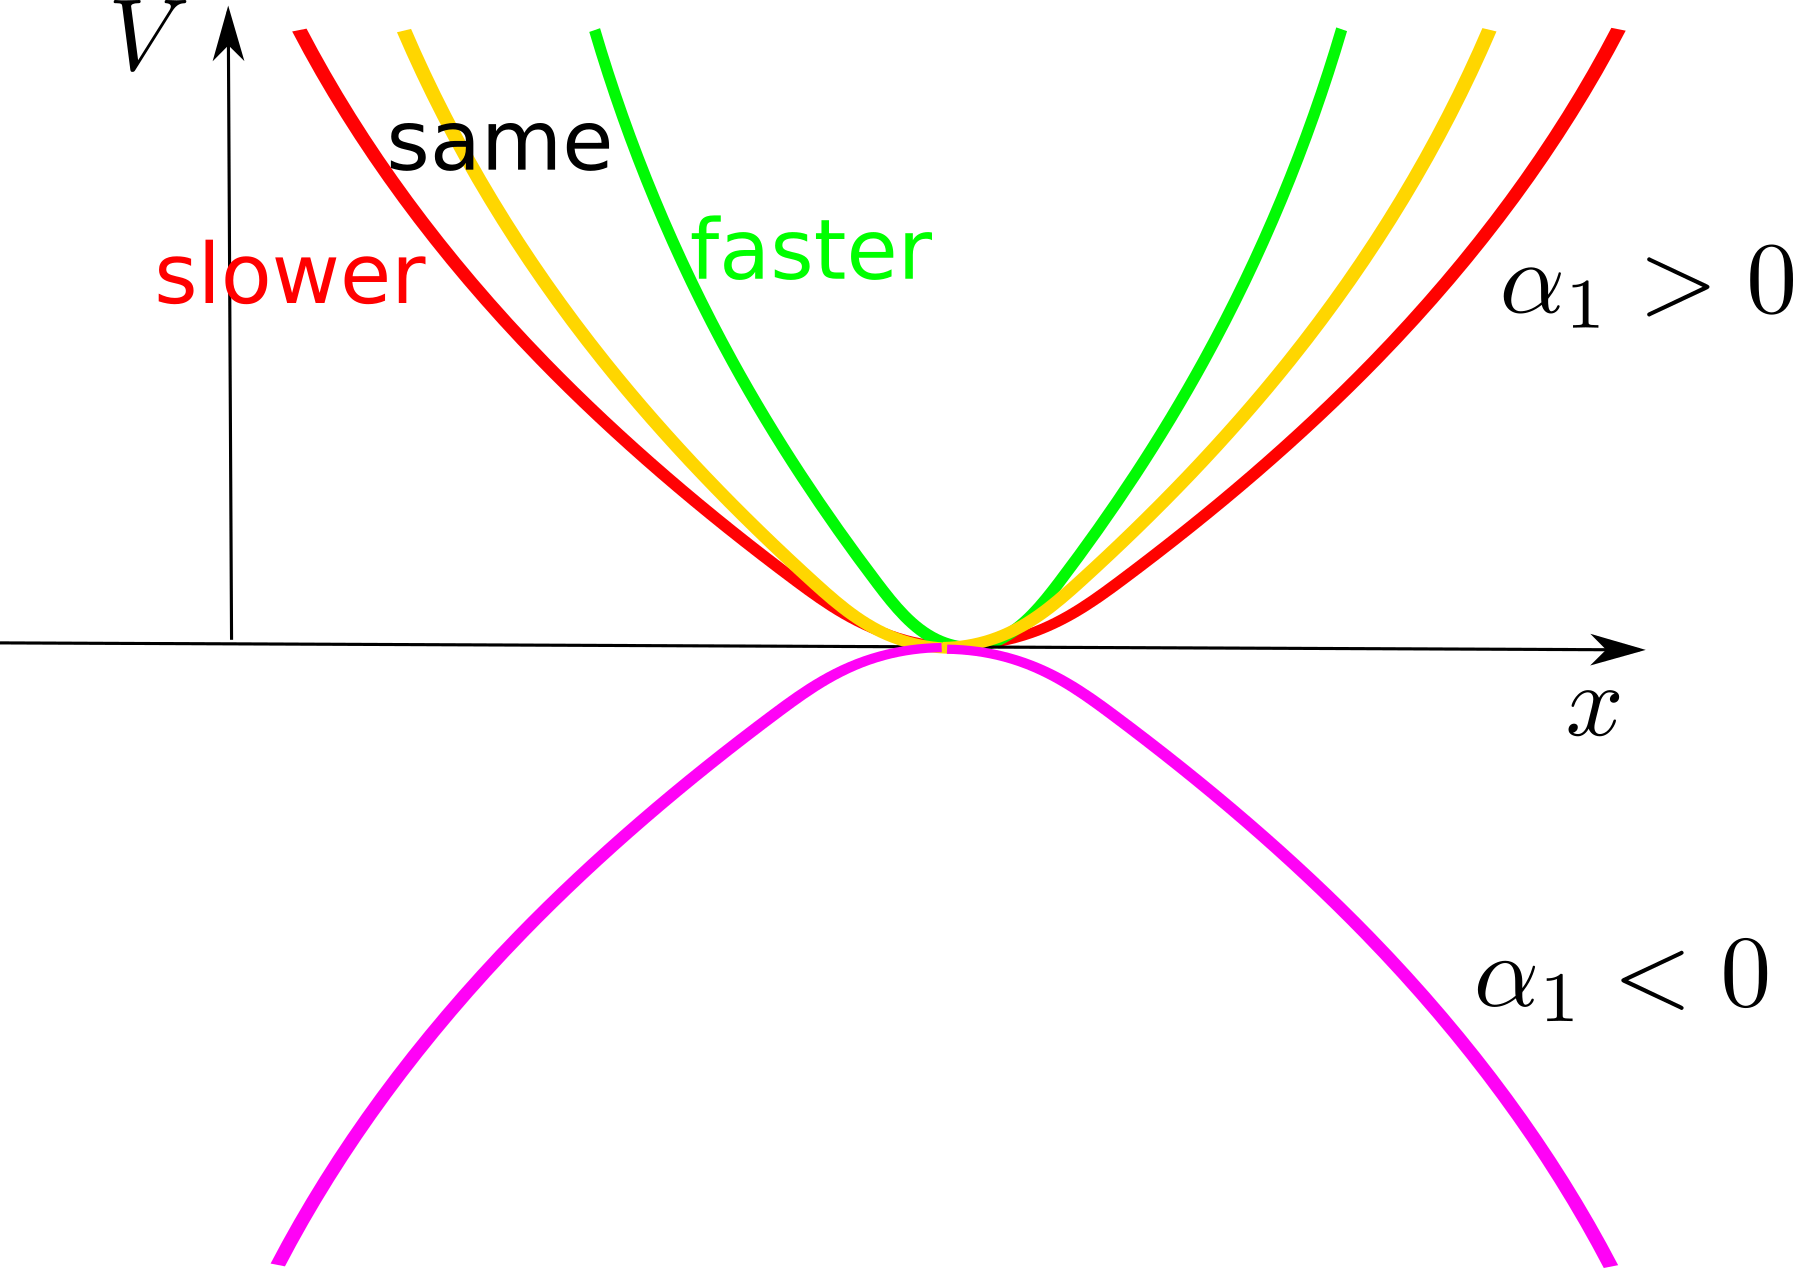
\includegraphics[width=2in]
{autoregulons/v-faster-same-slower.png}
\caption{$V(x)$ for 
$0<\alp_1<\alp$ (slower),
$\alp_1=\alp$ (same) and
$\alp_1>\alp$ (faster).
Also $V$ for $\alp_1<0$.}
\label{fig-v-low-high-pass}
\end{figure}
 
\end{enumerate}

\subsection{Linear Expansion of $h$}

In this section, we will
discuss the solution of
the autoregulon ODE
when $h(x)$ is replaced by
its linear approximation.

Let 

\beqa
\dot{x} &=& -\alp x + h_0 + h_1x
\\
&=& -\alp_1(x-x_a)
\eeqa
The most general solution of this ODE is

\beq
x(t)=\underbrace{\xi  e^{-\alp_1 t} }_{x_h}+
\underbrace{x_a\left[1-e^{-\alp_1 t}\right]}_{x_p}
\eeq
for some $\xi\in\RR$, as can be easily checked.
$x_h$ is called the {\bf homogeneous solution} (independent of $h$)\footnote{
$x_h$ satisfies the homogeneous ODE, i.e., the
ODE with $h(x)=0$.
}
and $x_p$ is called the {\bf particular solution} (dependent of $h$).
\footnote{
If we integrate both sides of
$\frac{dx}{h_0 -\alp_1 x}=dt$,
we only get the particular solution.}
From this general solution, we conclude that

\begin{itemize}
\item
\ul{if $\alp_1<0$, then:} $x(t)$ 
goes exponentially fast  from $\xi $ to $\pm \infty$,
growing as  $(\xi  -x_a)e^{|\alp_1|t}$
as $t\rarrow \infty$. 

\item \ul{if $\alp_1=0$, then:}
$x(t)$ is constant. 

\item 
\ul{if $\alp_1>0$, then:} $x(t)$ goes exponentially fast from
$\xi $ to $x_a$ as $t\rarrow \infty$.
As illustrated in Fig.\ref{fig-fast-normal-slow}, in
this case,
we can have a convergence rate (CR)
 to $x_a$
 that is either faster, the same or slower than $\alp$:
\begin{itemize}[$\checkmark$]

\item \ul{if $0<h_1<\alp$, then:} $\alp_1<\alp$, 
CR is slower than $\alp$, {\bf positive autoregulation (PAR)}, positive feedback

\item \ul{if $h_1=0$, then:} $\alp_1=\alp$, CR is same as $\alp$,
{\bf zero autoregulation (ZAR)}

\item \ul{if $h_1<0$, then:} $\alp_1>\alp$, CR is faster than $\alp$,
{\bf negative autoregulation (NAR)},
negative feedback
\end{itemize}
\end{itemize}


\begin{figure}[h!]
\centering
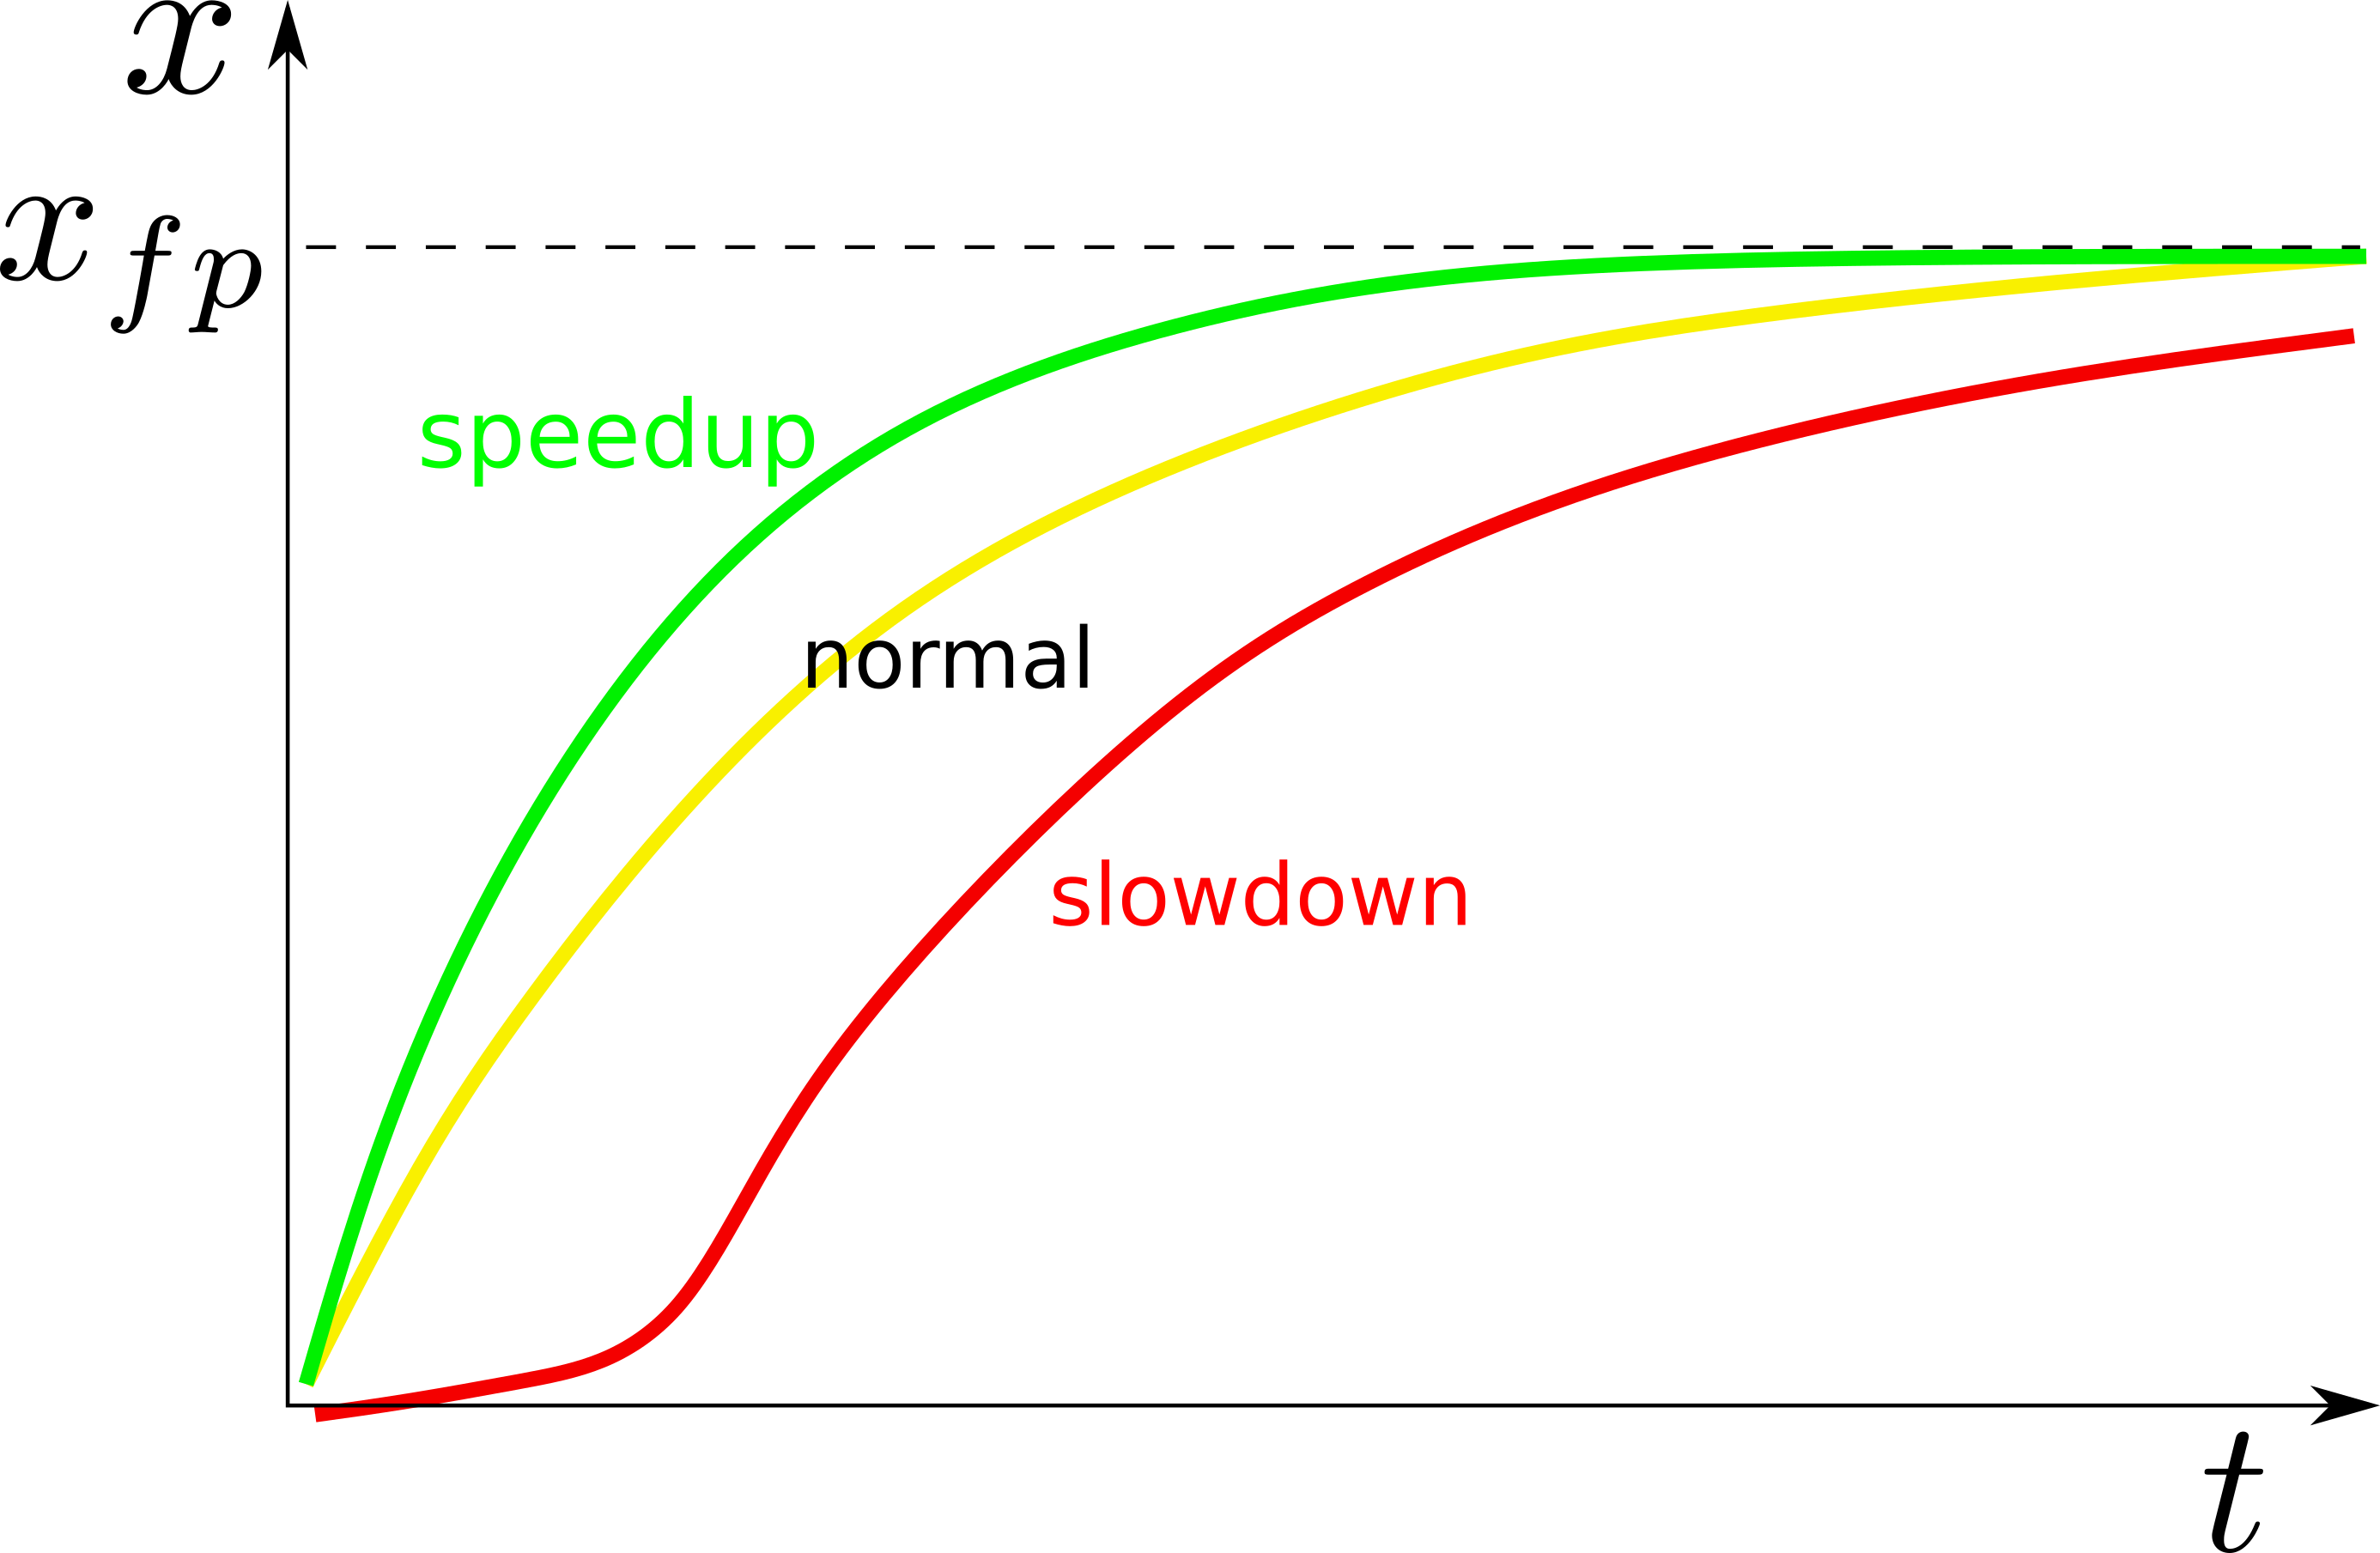
\includegraphics[width=2.5in]
{autoregulons/fast-normal-slow.png}
\caption{For a single autoregulon
with $\alp_1>0$, the convergence rate to $x_a$ can 
be either faster, the same or slower than $\alp$.
 }
\label{fig-fast-normal-slow}
\end{figure}




\subsection{Lowpass $h$}

In this section, we will
discuss the solution of
the autoregulon ODE
when $h(x)$ is
an ideal lowpass filter.

Let 

\beq
\dot{x} = -\alp x + \beta\indi(x<K)
\eeq
where $\beta, \alp, K>0$. Then

\beq
x= 
\left\{
\begin{array}{ll}
\xi  e^{-\alp t} +
\frac{\beta}{\alp}\left[1-e^{-\alp t}\right]
&\text{ if } x<K
\\
K e^{-\alp (t-t_K)}
&\text{ if } x>K
\end{array}
\right.
\eeq
for some $\xi\in\RR$. To make $x(t)$ continuous at $t=t_K$ when $x=K$,
we must have

\beq
 \xi  e^{-\alp t_K} +
\frac{\beta}{\alp}
\left[1-e^{-\alp t_K}\right]
=
K
\eeq


\begin{figure}[h!]
\centering
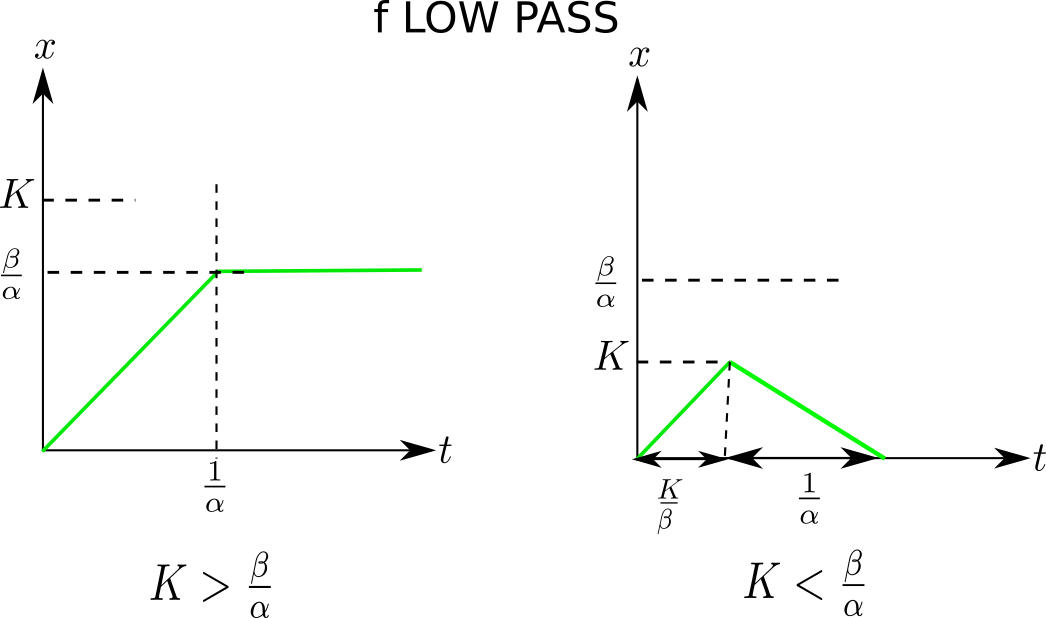
\includegraphics[width=4in]
{autoregulons/autoreg-lowpass.png}
\caption{Approximate $x(t)$
for an autoregulon with a lowpass $h$
and $x(0) =0$}
\label{fig-autoreg-lowpass}
\end{figure}

See Fig.\ref{fig-autoreg-lowpass}
for a plot of the approximate 
$x(t)$ for an autoregulon with a lowpass $h$
and $x(0) =0$.

Note that if $\alp t<<1$, then\footnote{Use $e^x\approx 1 + x$ for $|x|<<1$.}, 

\beqa
x &\approx&
\left\{
\begin{array}{ll}
\xi  + (\beta -\alp \xi )t
&
\text{if }x<K
\\(1-\alp t)
Ke^{\alp t_K}
&
\text{if }x>K
\end{array}
\right.
\eeqa

Assume $x(0)=\xi =0$ for simplicity.
In that case, $x$
increases monotonically towards $\frac{\beta}{\alp}$. 
If $K>\frac{\beta}{\alp}$,
then $x$ reaches $\frac{\beta}{\alp}$
without ever passing through $K$.
So $x(t)$ remains in the $x<K$ branch of the
the solution throughout. 
On the other hand, if $K<\frac{\beta} {\alp}$, 
when $x$ reaches $K$ and tries to
switch branch, it can't do it because
$\partial_x^2V(x)>0$ for $x=K\pm \eps$
so $\dot{x}=0$ at $x=K$.






\subsection{Highpass $h$}

In this section, we will
discuss the solution of
the autoregulon ODE
when $h(x)$ is
an ideal highpass filter.

Let 

\beq
\dot{x} = -\alp x + \beta\indi(x>K)
\eeq
where $\beta, \alp, K>0$. Then

\beq
x= 
\left\{
\begin{array}{ll}
K e^{-\alp (t-t_K)} &\text{ if } x<K 
\\
\xi  e^{-\alp t} +
\frac{\beta}{\alp}
\left[ 1-e^{-\alp t}\right]
&\text{ if } x>K
\end{array}
\right.
\eeq
for some $\xi\in\RR$. To make $x(t)$ continuous at $t=t_K$ when $x=K$,
we must have

\beq
K=\xi e^{-\alp t_K}+\frac{\beta}{\alp}
\left[ 1-e^{-\alp t_K}\right]
\label{eq-x0-K-prop}
\eeq

\begin{figure}[h!]
\centering
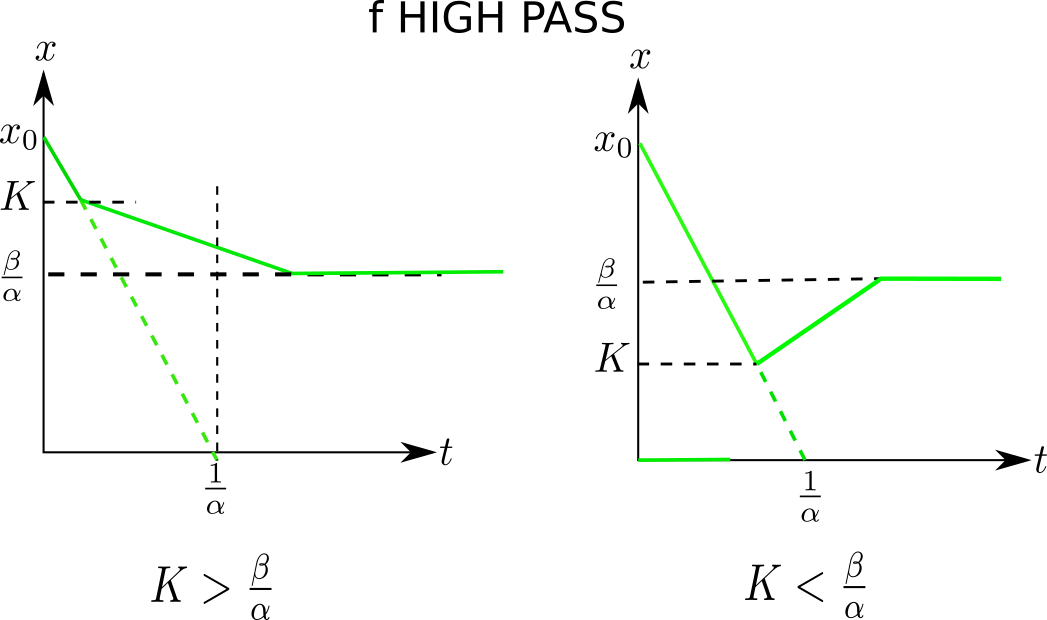
\includegraphics[width=4in]
{autoregulons/autoreg-highpass.png}
\caption{Approximate $x(t)$ for an autoregulon with a highpass $h$
and $x(0)>K$.}
\label{fig-autoreg-highpass}
\end{figure}

See Fig.\ref{fig-autoreg-highpass}
for a plot of the approximate 
$x(t)$ for an autoregulon with a highpass $h$
and $x(0) >K$.

Note that if $\alp t<<1$, then\footnote{Use $e^x\approx 1 + x$ for $|x|<<1$.}, 

\beqa
x &\approx&
\left\{
\begin{array}{ll}
(1-\alp t)
Ke^{\alp t_K}
&
\text{if }x<K
\\
\xi  + (\beta -\alp \xi )t
&
\text{if }x>K
\end{array}
\right.
\eeqa

Unlike when $h$ is a lowpass
filter, 
in this case,
assuming $x(0)=0$ is boring, because $x(t)$
remains at $0$. 
Assume
$x(0) >K$ instead. 

If $K<\frac{\beta}{\alp}$,
$x(t)$ remains always in the $x>K$
branch and plateaus at $x=\frac{\beta}{\alp}$.

If $K> \frac{\beta}{\alp}$,
$x(t)$ switches from the $x>K$ branch to
the $x<K$ branch, and then decays to zero.









\subsection{Fixed Points}

The fixed points of an autoregulon satisfy

\beq
0=\dot{x}=-\alp x + h(x)
\eeq
Thus, they occur whenever the curves
$y=\alp x$ and $y=h(x)$ intersect. When $h(x)$ is 
a straight line as in positive or negative
feedback, there is just one intersection. But when
$h(x)$ is a Hill function,
$y=\alp x$ and $y=h(x)$ can intersect at 1, 2 or 3 points.
Fig.\ref{fig-source-sink-source} shows 
the case where there are 3 intersections, leading to 3 fixed points,
one source and two sinks.

\begin{figure}[h!]
\centering
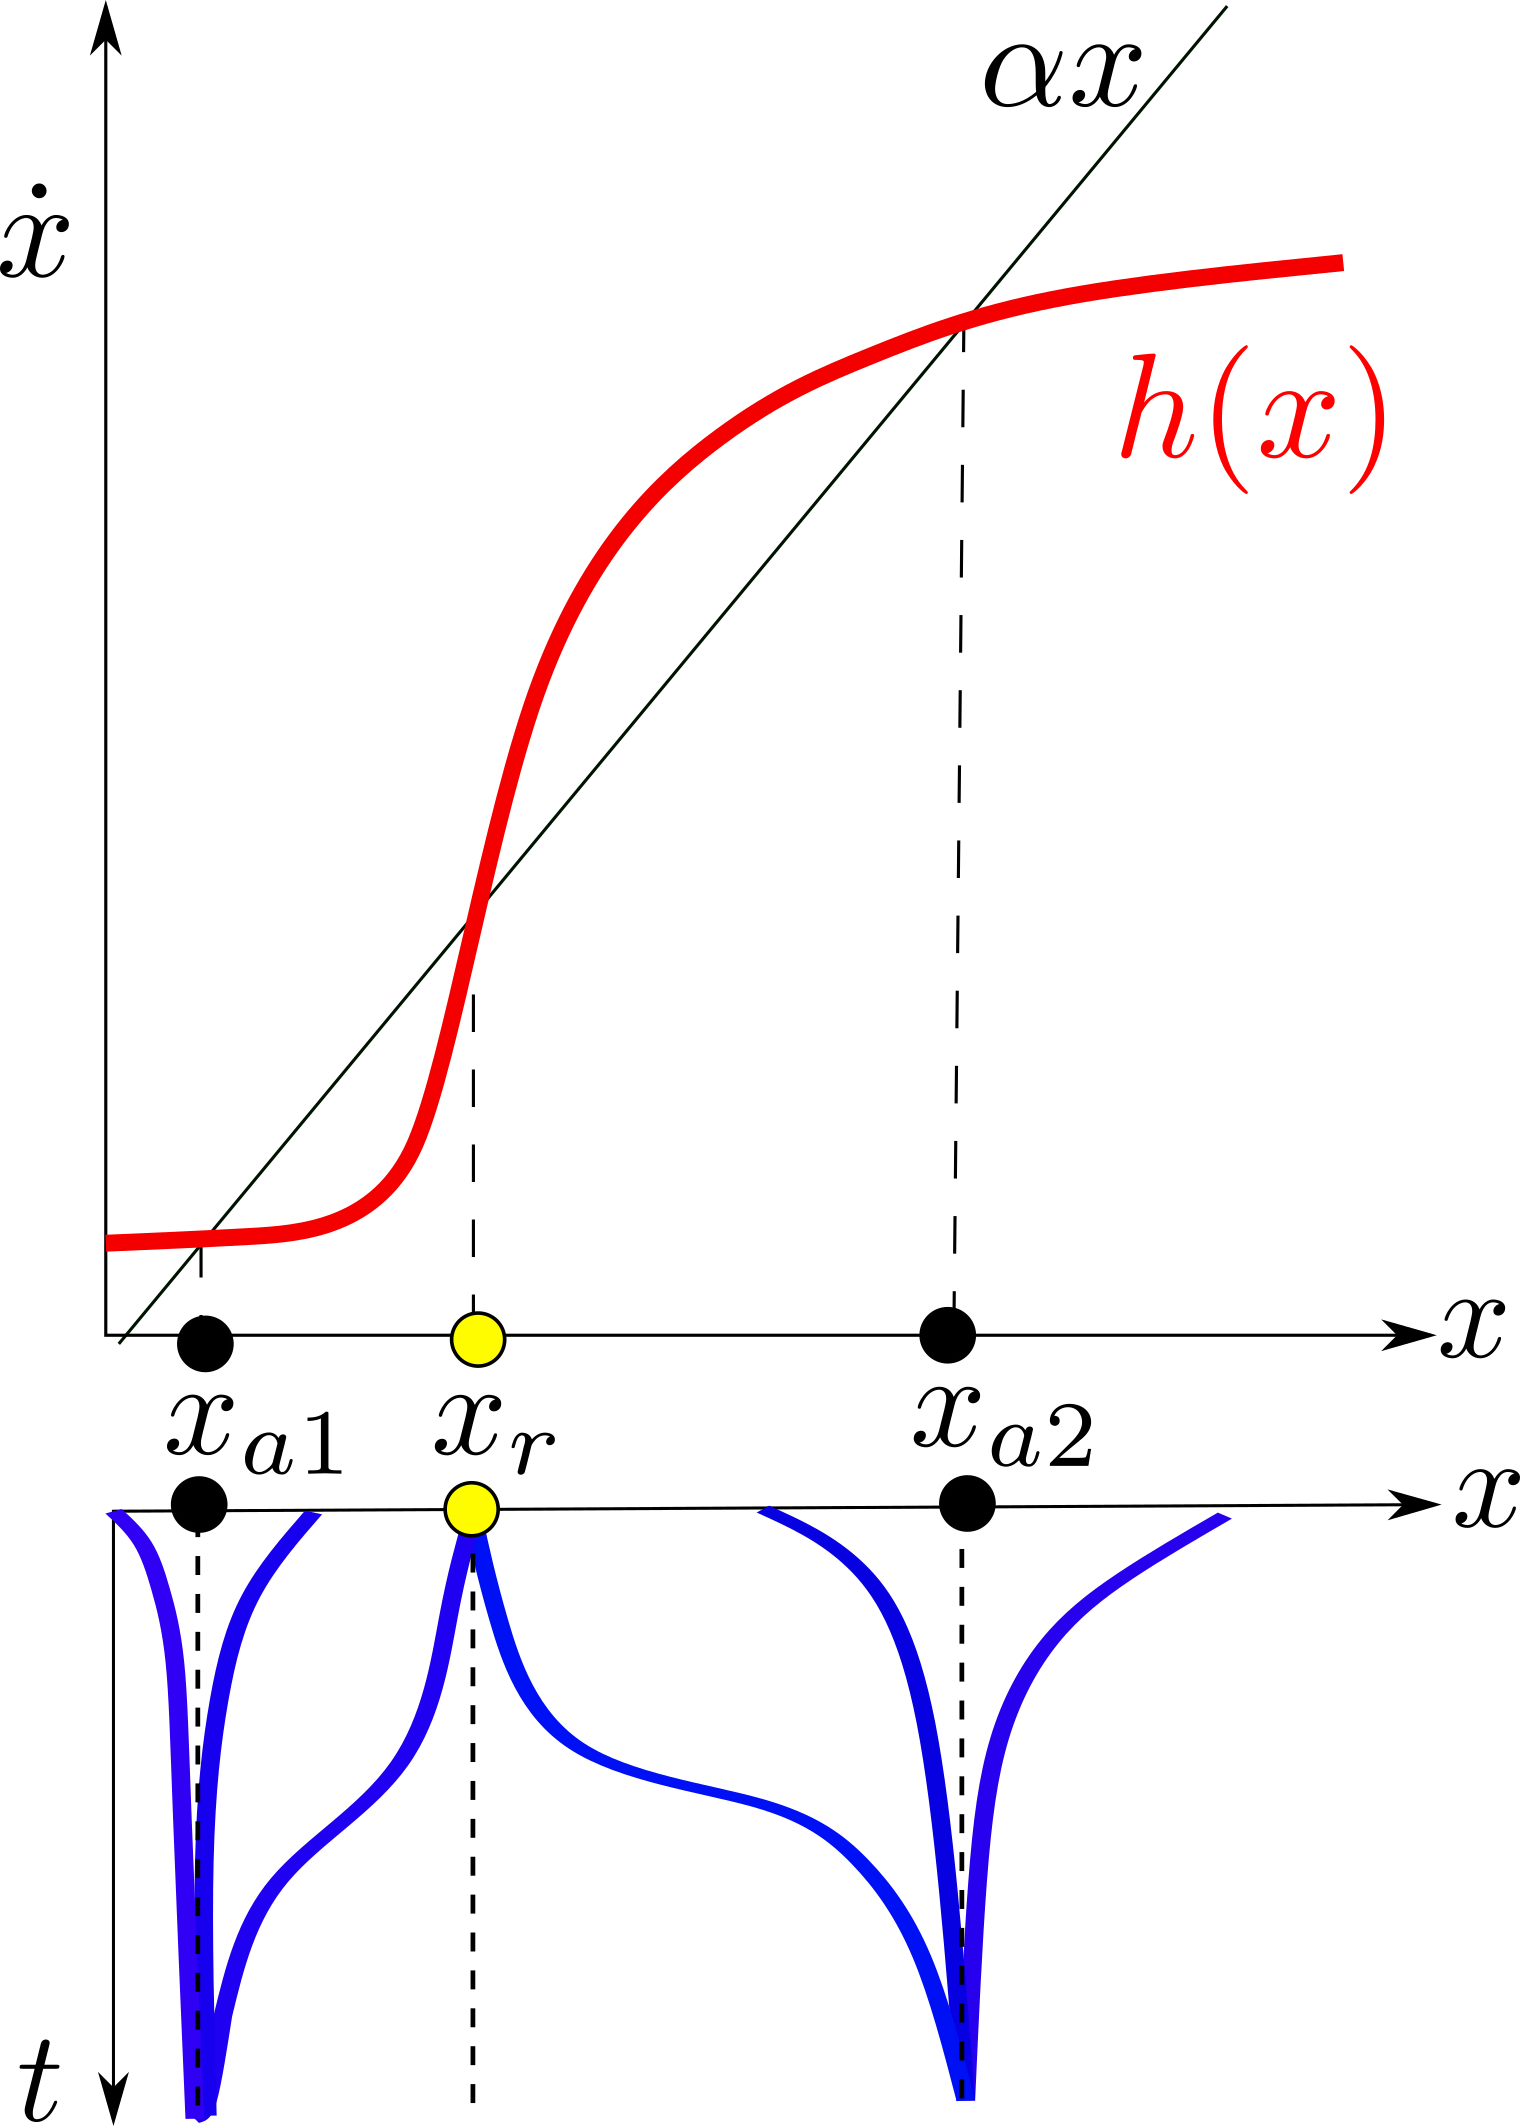
\includegraphics[width=2in]
{autoregulons/source-sink-source.png}
\caption{For single autoregulon $\dot{x}(t)=-\alp x + h(x)$, 
the fixed points occur at the intersection of the
curves $y=\alp x$ and $y=h(x)$. In this case,
there are 3 intersections, leading to 3 fixed points.
}
\label{fig-source-sink-source}
\end{figure}



\section{Two autoregulons}

\begin{figure}[h!]
\centering
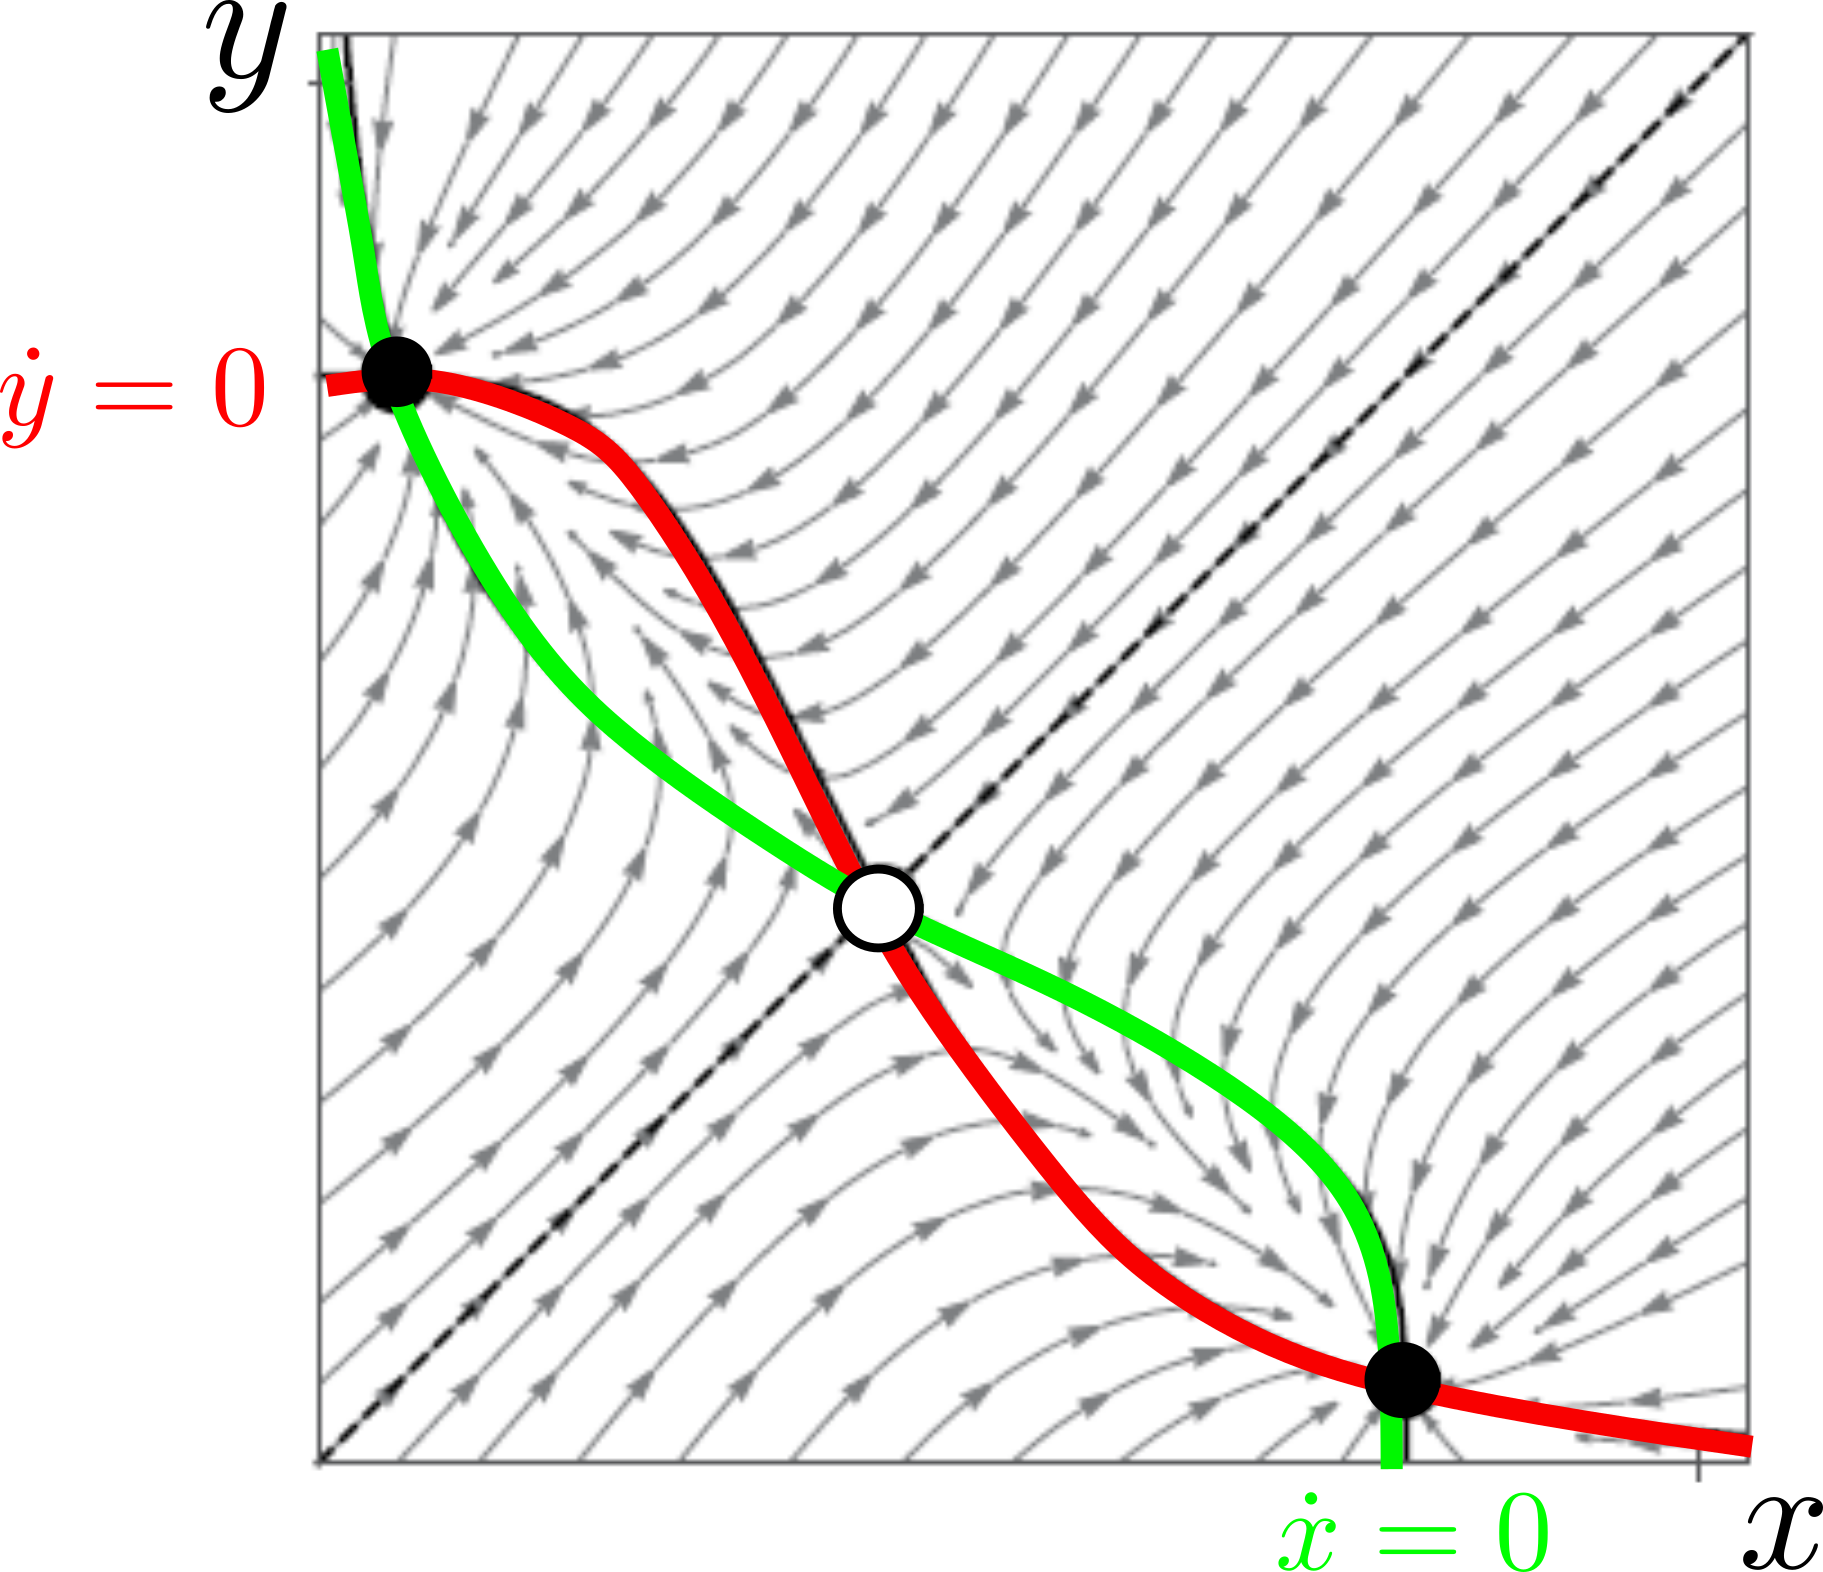
\includegraphics[width=3in]
{autoregulons/2dim-3fp.png}
\caption{Phase portrait
for two autoregulon with 3 fixed
points.}
\label{fig-2dim-3fp}
\end{figure}


\beq
\begin{array}{c}
\xymatrix@C=6pc@R=1pc{
\rvx \ar@{=>}[dd]\ar[ddr]|<<<<{}
& \rvy \ar@{=>}[dd]\ar[ddl]|<<<<{}
\\
&
\\
\dot{\rvx}
&\dot{\rvy}
}
\xymatrix{\\
\quad=\quad}
\xymatrix@C=5pc{
\\
\Rect{\rvx}
\fbackar{r}
{}
{}
&
\Rect{\rvy}}
\\
\left\{
\begin{array}{l}
\dot{x}=
\\
\dot{y}=
\end{array}
\right.
\end{array}
\eeq

Two autoregulons connected to each other.




\beq
\begin{array}{c}
\xymatrix@C=4pc@R=1pc{
\rvx \ar@{=>}[dd]\ar[ddrr]|<<<<{}
\ar[r]
&\bigotimes\ar[ddl]\ar[ddr]
& \rvy \ar@{=>}[dd]\ar[ddll]|<<<<{}
\ar[l]
\\
&
\\
\dot{\rvx}
&
&\dot{\rvy}
}\quad
\xymatrix{\\
\quad=\quad}
\xymatrix@R=4pc@C=3pc{
\Rect{\rvx}\widefbackar{rr}{}{}
\fbackar{r}{}{}
&\bigotimes\fbackar{r}{}{}
&\Rect{\rvy}
}
\\
\left\{
\begin{array}{l}
\dot{x}=
\\
\dot{y}=
\end{array}
\right.
\end{array}
\eeq




Two autoregulons connected to each other, including population product (pp) term.


feedback

\subsection{Two Autoregulon Negative Feedback}


Net for Two Autoregulon Negative Feedback (2AR-NF)

\beq
\xymatrix@C=5pc
{\Rect{\rvx}
\fbackar{r}{\redminus}{\redplus}
&\Rect{\rvy}
}
\quad
\left\{
\begin{array}{l}
\dot{x}=-\alp_1 x - \gamma_1 y
\\
\dot{y}= -\alp_2y + \gamma_2 x
\end{array}
\right.
\eeq

\subsection{Two autoregulon Positive Feedback}

\beq
\begin{array}{ccc}
(a)
&\xymatrix@C=5pc
{\Rect{\rvx}
\fbackar{r}{\redminus}
{\redminus}
&\Rect{\rvy}
}
&
\left\{
\begin{array}{l}
\dot{x}=-\alp_1 x - \gamma_1 y
\\
\dot{y}= -\alp_2y - \gamma_2 x
\end{array}
\right.
\\
\\
(b)&
\xymatrix@C=5pc
{\Rect{\rvx}
\fbackar{r}{\redplus}
{\redplus}
&\Rect{\rvy}
}
&
\left\{
\begin{array}{l}
\dot{x}=-\alp_1 x + \gamma_1 y
\\
\dot{y}= -\alp_2y + \gamma_2 x
\end{array}
\right.
\end{array}
\eeq

Net for 2 Autoregulon Positive Feedback (2AR-PF)

\subsection{Genetic Toggle Switch}
A  {\bf genetic toggle switch}
can be described by:

Genetic Toggle Switch. \OTO\cite{OTO}


\beq
\xymatrix@C=3pc@R=4pc{
\rvx\ar[dr]|\redominus
\ar[d]|\redminus
&\rvy\ar@/_1pc/[dl]|\redominus
\ar[d]|\redminus
\\
\dot{\rvx}
&\dot{\rvy}
}
\left\{
\begin{array}{l}
\dot{x} = \frac{\alpha_1}{1 + \left(\frac{y}{K_1}\right)^{n_1}} - \gamma_1 x
\\
 \dot{y} = \frac{\alpha_2}{1 + \left(\frac{x}{K_2}\right)^{n_2}} - \gamma_2 y
\end{array}
\right.
\eeq

where $x$, $y$, and $z$ represent concentrations of proteins, $\alpha_1, \alpha_2, \alpha_3 > 0$ are production rates, and $n, m, p > 1$ control the steepness of the repression.


\section{More than 2 autoregulons}


\begin{figure}[h!]
$$
\begin{array}{ccc}
\xymatrix@C=3pc@R=5pc{
&\Rect{\rvx}
\fbackar{ld}{}{}
\fbackar{rd}{}{}
\\
\Rect{\rvy}\fbackar{rr}{}{}
&&
\Rect{\rvz}
}
&
\xymatrix@C=3pc@R=5pc{
&\Rect{\rvx}
\fbackar{ld}{-}{0}
\fbackar{rd}{+}{0}
\\
\Rect{\rvy}\fbackar{rr}{-}{0}
&&
\Rect{\rvz}
}
&
\xymatrix@C=3pc@R=5pc{
&\Rect{\rvx}
\fbackar{ld}{-}{0}
\fbackar{rd}{+}{0}
\\
\Rect{\rvy}\fbackar{rr}{+}{0}
&&
\Rect{\rvz}
}
\\
\\
(a)&(b)&(c)
\end{array}
$$
\caption{$(a)$ shows a coherent net of 3 autoregulons because $\sign(\gamma_{\rvy\rarrow\rvz}\gamma_{\rvx\rarrow\rvy})=\sign(\gamma_{\rvx\rarrow\rvz})$.
$(b)$ shows an incoherent net of 3 autoregulons because $\sign(\gamma_{\rvy\rarrow\rvz}\gamma_{\rvx\rarrow\rvy})\neq \sign(\gamma_{\rvx\rarrow\rvz})$.
}
\label{fig-3-coherent-autoregulons}
\end{figure}





\begin{figure}
$$
\begin{array}{ccccc}
\xymatrix{
&\Rect{\rvx}\ar[dl]
\ar[dr]
\\
\Rect{\rvy}\ar[rr]
&&\Rect{\rvz}
}&
&
\xymatrix{
&\Rect{\rvx}\ar[dl]|\redoplus
\ar[dr]|\redoplus
\\
\Rect{\rvy}\ar[rr]|\redoplus
&&\Rect{\rvz}
}
&
&
\xymatrix{
&\Rect{\rvx}\ar[dl]|\redoplus
\ar[dr]|\redoplus
\\
\Rect{\rvy}\ar[rr]|\redominus
&&\Rect{\rvz}
}
\\
(a)
&&(b)
&&(c)
\end{array}
$$
\caption{$(a)$ Forward Feed Loop (FFL) net.
$(b)$ Coherent Type 1 FFL (C1-FFL).
$(c)$ Incoherent Type 1 FFL (I1-FFL)}
\end{figure}

\beq
\xymatrix{
&&\Rect{\rvx}
\fbackar{ddll}{\oplus}{0}
\ar[dl]
\\
&\bigotimes
\ar@/_1pc/[drr]|\redplus
\\
\Rect{\rvy}\ar[ur]|\redoplus
&&&\Rect{\rvz}
}
\quad
\left\{
\begin{array}{l}
\dot{x}=
\\
\dot{y} =-\alp_\rvy y + \beta_\rvy
h_\oplus(x)
)
\\
\dot{z} = -\alp_\rvz z + \beta_\rvz 
h_\oplus(x)h_?(y)
\end{array}
\right.
\eeq


Feedforward Loop (FFL).

Coherent/Incoherent Type 1 FFL (C1-FFL/I1-FFL) if $K_{\rvy\rarrow\rvz}$ is highpass/lowpass.
where parameters (i.e., $\alp_\rvy, \alp_\rvz, \beta_\rvy, \beta_{\rvz}$) are positive.




\subsection{C1-FFL}

\beq
\xymatrix{
\rvx \ar@/_1pc/[drr]|\redoplus
\ar[r]|\redoplus
&\bigotimes\ar@/_3pc/[drr]|{\redplus}
& \rvy\ar[d]|{\redminus}\ar[l]|
\redoplus
&\rvz\ar[d]|{\redminus}
\\
&
& \dot{y}
&
\dot{z} 
}
\left\{
\begin{array}{l}
\dot{y} =-\alp_\rvy y + \beta_\rvy \indi(x>K_{\rvx\rarrow\rvy}
)
\\
\dot{z} = -\alp_\rvz z + \beta_\rvz \indi(x> K_{\rvx\rarrow\rvz})
{\color{red}\indi(y>K_{\rvy\rarrow\rvz})}
\end{array}
\right.
\eeq

\begin{figure}[h!]
\centering
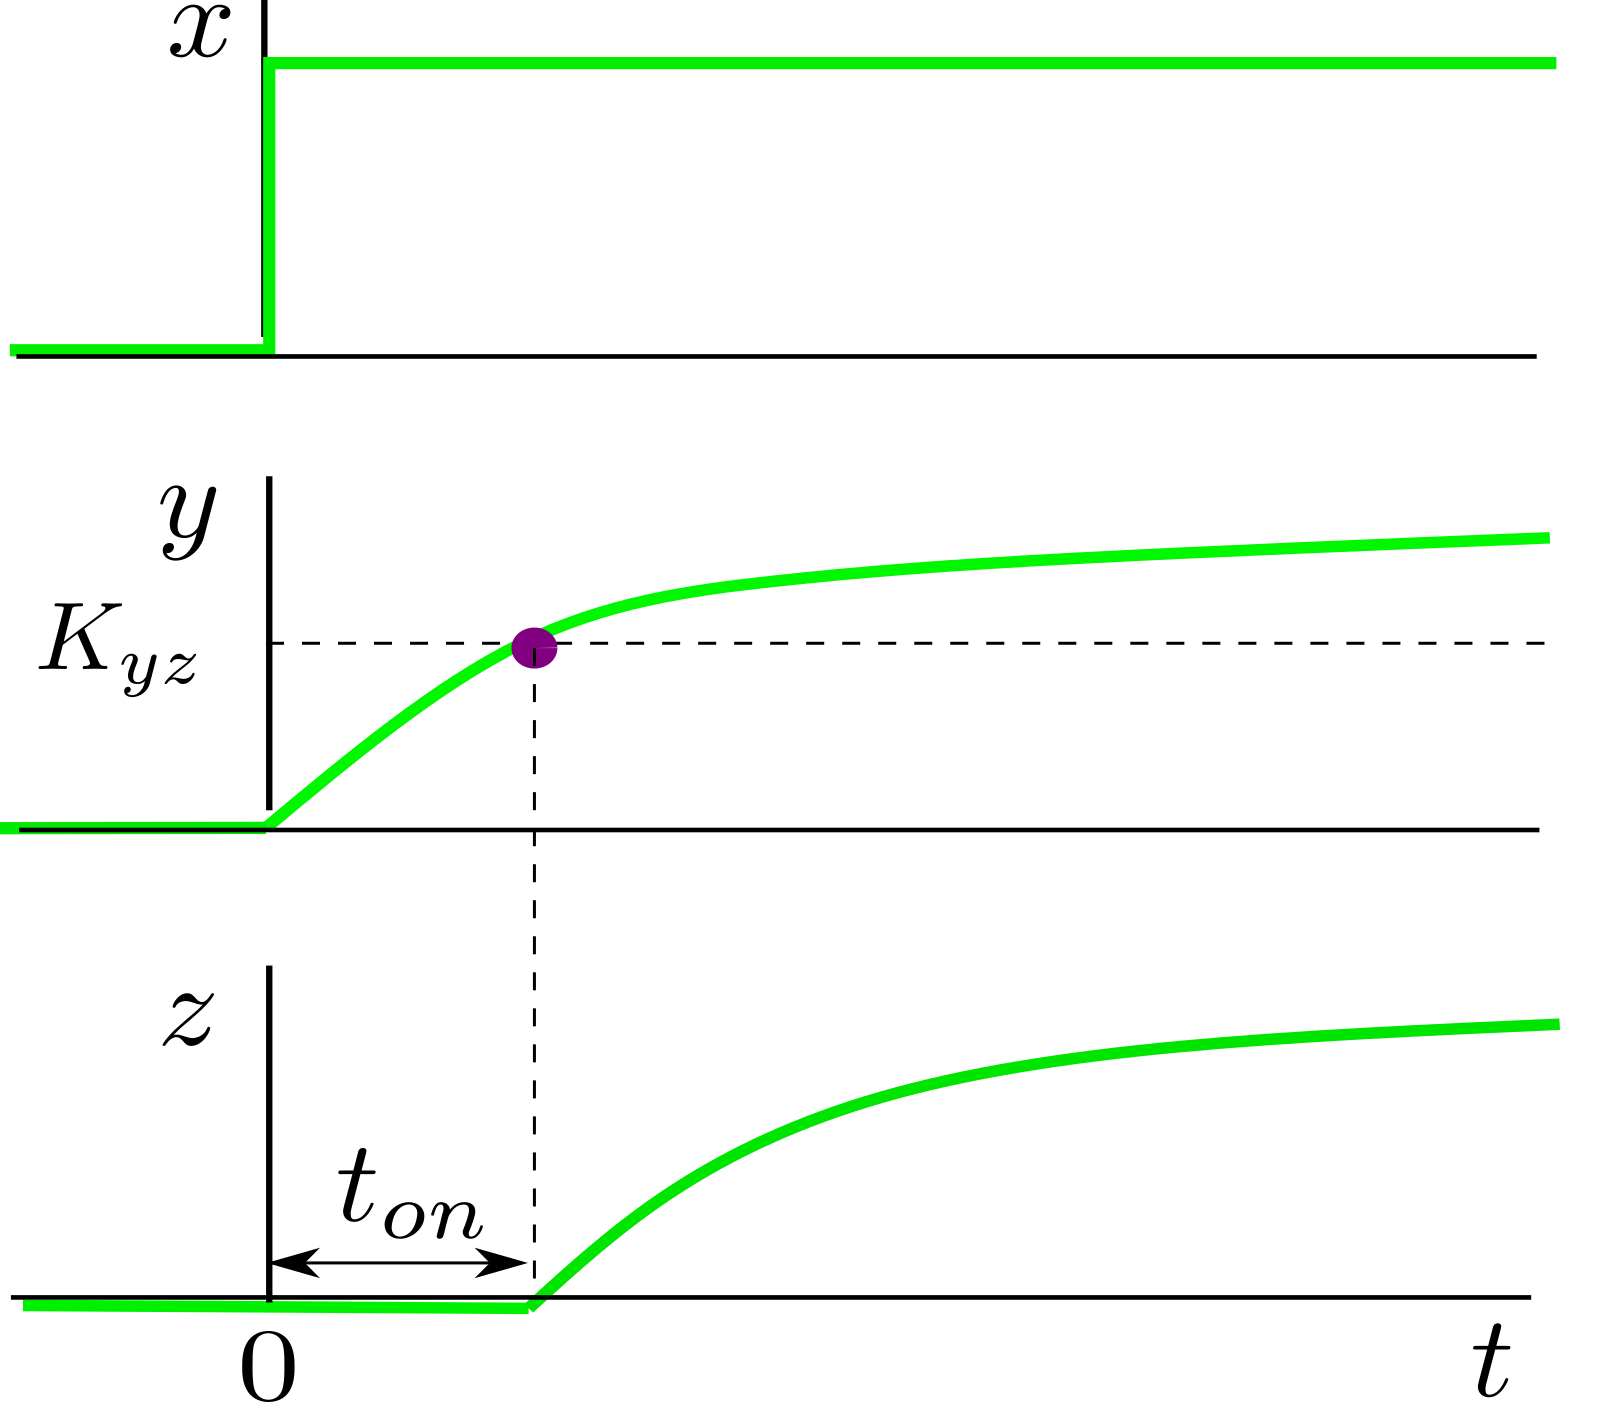
\includegraphics[height=2in]
{autoregulons/c1-ffl-up-green.png}
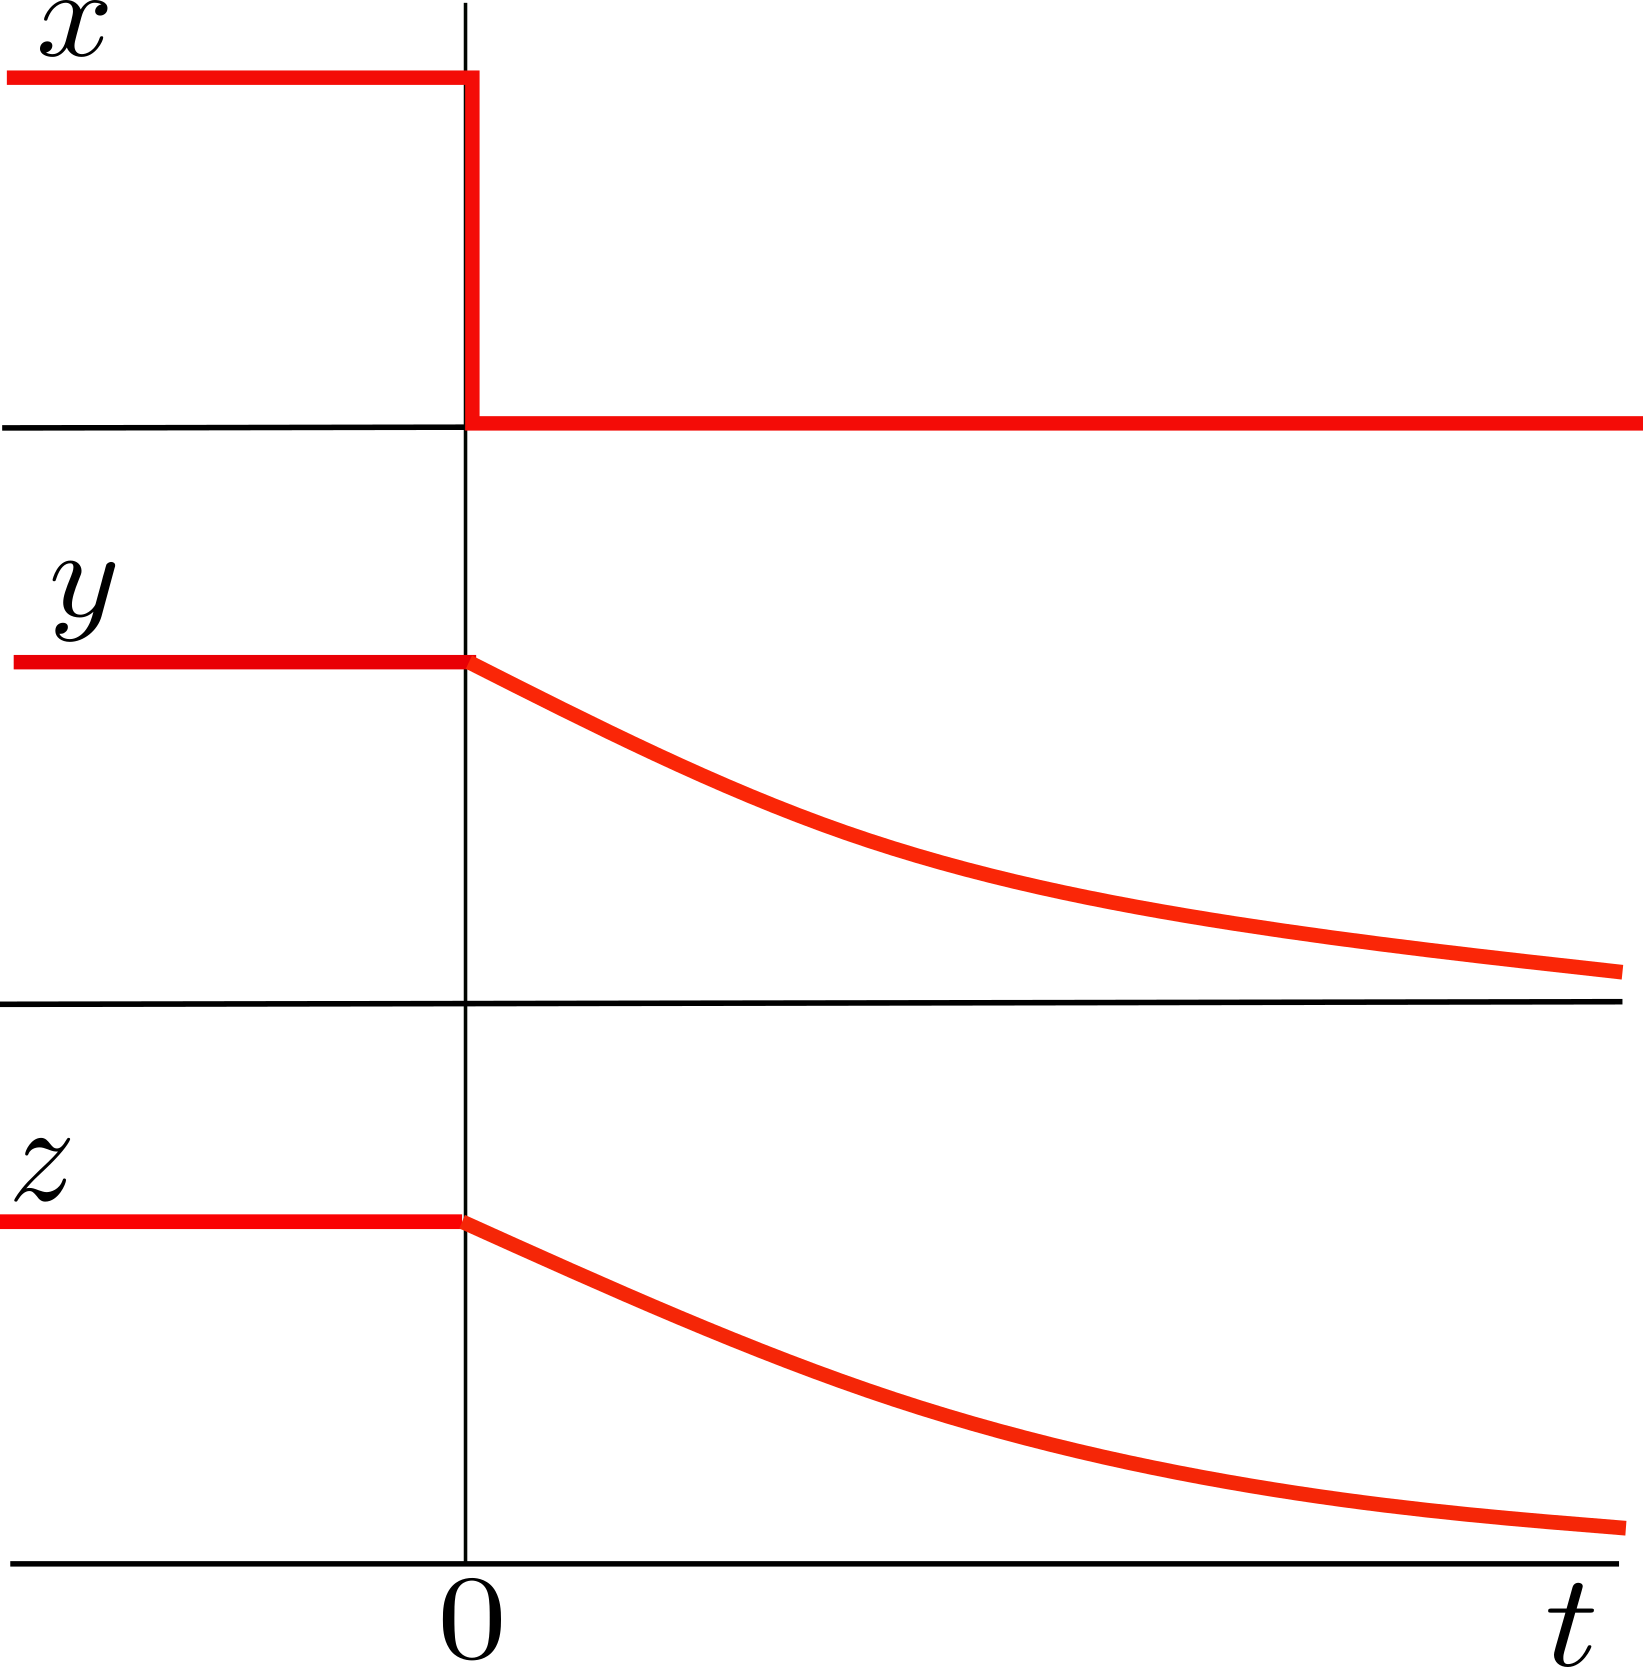
\includegraphics[height=2in]
{autoregulons/c1-ffl-down-green.png}
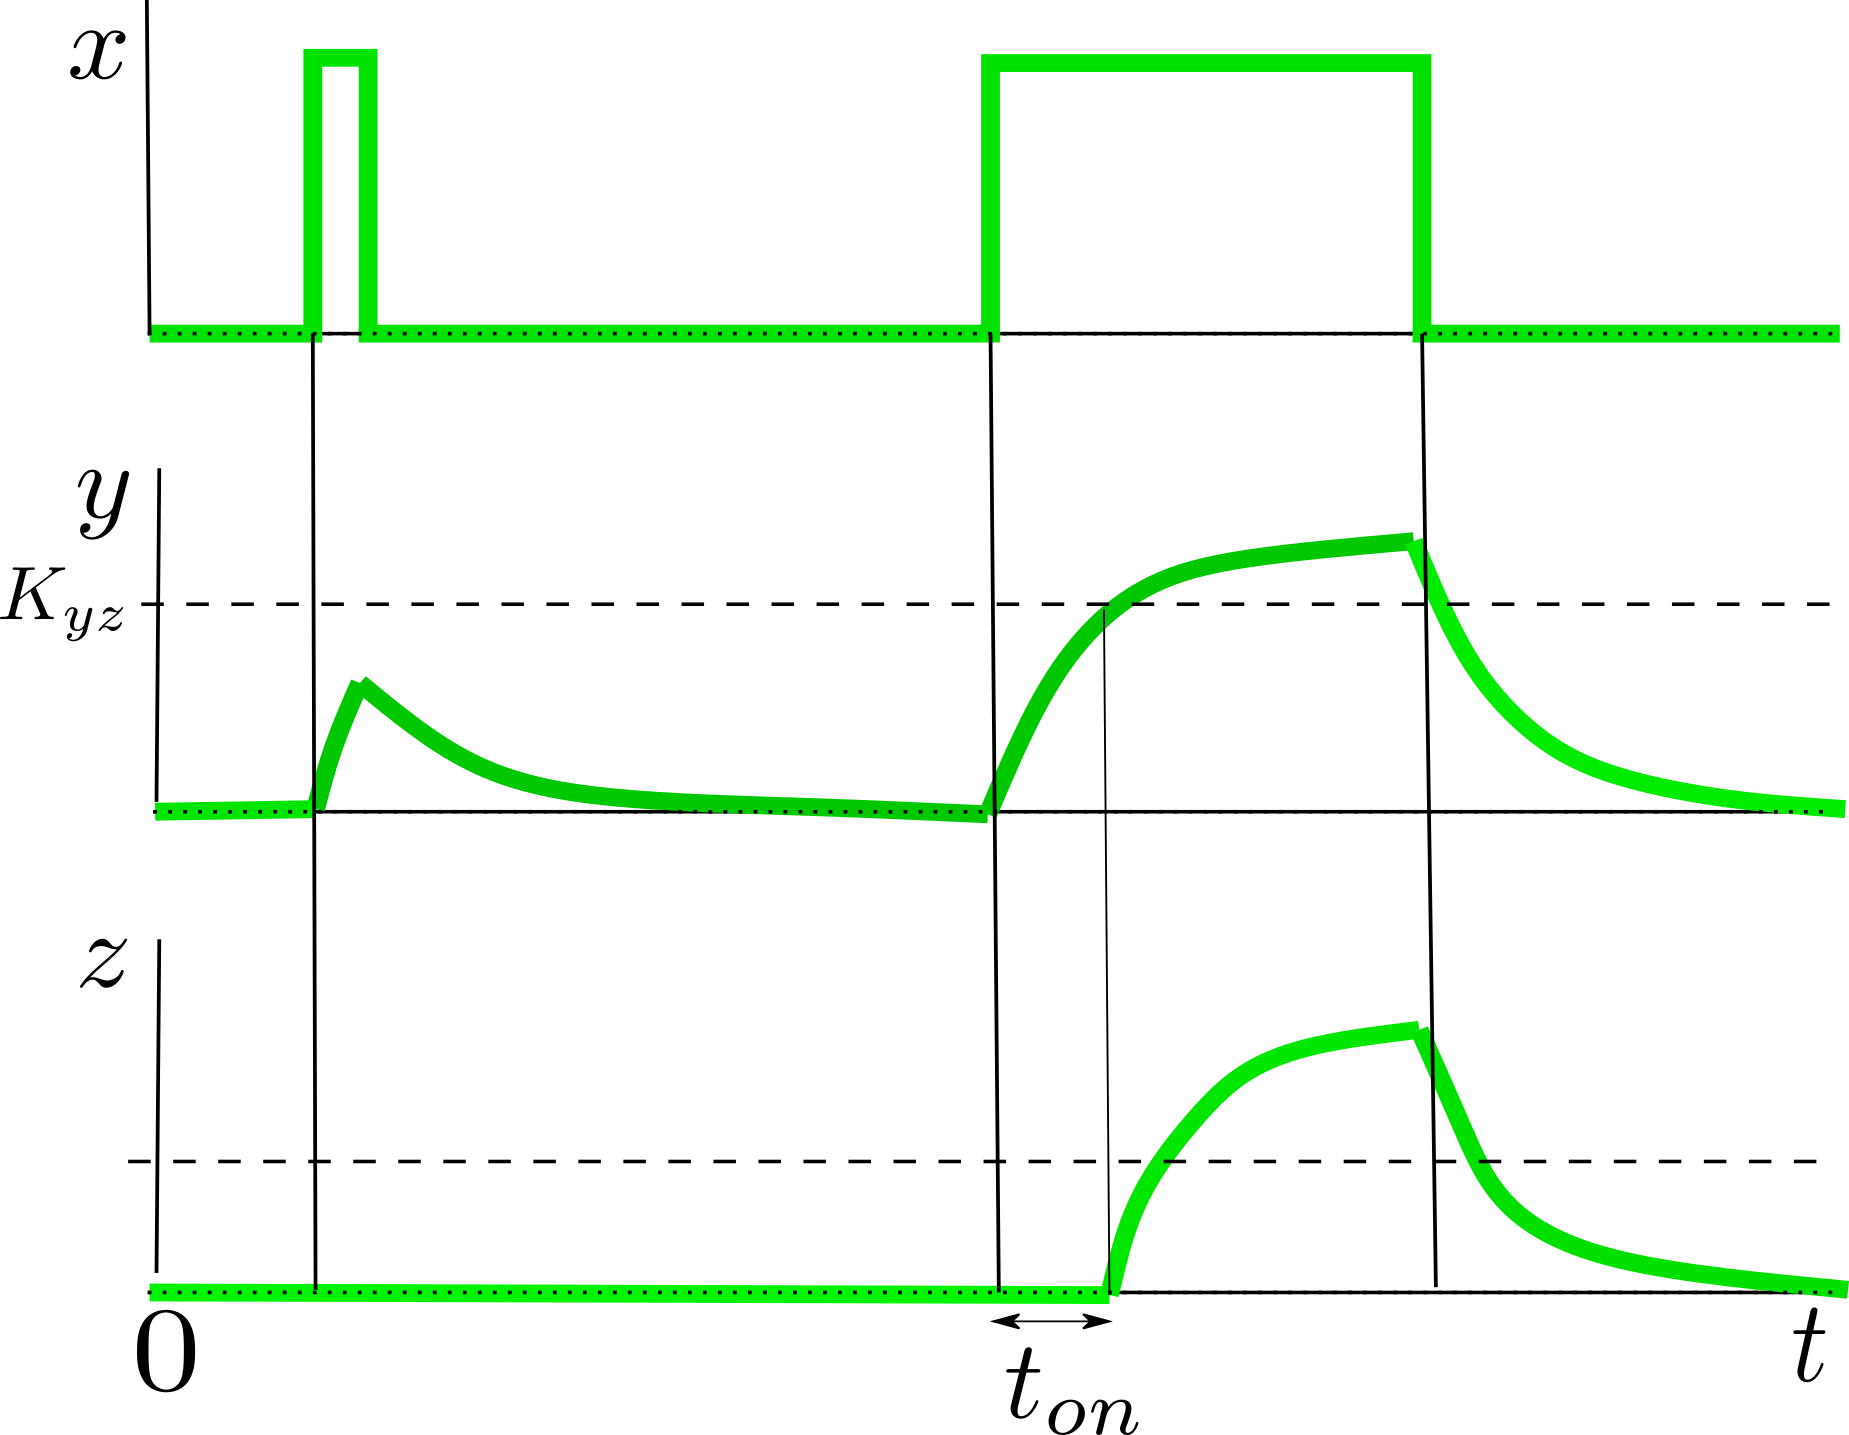
\includegraphics[height=2in]
{autoregulons/c1-ffl-up-down-green.png}
\caption{For C1-FFL, $x(t)$, $y(t)$, $z(t)$ assuming 
that $x(t)$ is either a rising step function (in green),
a dropping step function (in red),
or a square impulse function (in purple).}
\label{fig-c1-ffl-triple}
\end{figure}


Below, the red equations 
correspond to a different choice of $x(t)$.

Assume (see Fig.\ref{fig-c1-ffl-triple})
\beq
x = \xi \indi(t>0)
\eeq
\beq \nonumber
\color{red}
x = \xi \indi(t<0)
\eeq
where $\xi  > K_{\rvx\rarrow\rvy}, K_{\rvx\rarrow\rvz}$.
Thus, Eq.(\ref{eq-ffl-gen}) reduces to

\beq
\left\{
\begin{array}{l}
\dot{y} = \beta_\rvy
-\alp_\rvy y
\\
\dot{z} =  \beta_\rvz
\indi(y>K_{\rvy\rarrow\rvz}) -\alp_\rvz z
\end{array}
\right.
\label{eq-ffl-red}
\eeq
Let $
y(0) = 0, y_{ss} = \frac{\beta_\rvy}{\alp_{\rvy}}
$.\
Then (see Fig.\ref{fig-c1-ffl-triple})

\beq
y = y_{ss}(1-e^{-\alp_\rvy t})
\eeq
\beq \nonumber \color{red}
y = y_0e^{-\alp_\rvy t}
\eeq
If $y_{ss}> K_{\rvy\rarrow\rvz}$
( or ${\color{red} y_0 < K_{\rvy\rarrow\rvz}}$), then (see Fig.\ref{fig-c1-ffl-triple})


\beq
z = \frac{\beta_\rvz}{\alp_\rvz}(1- e^{-\alp_\rvz (t-t_{on})})
\eeq
\beq\nonumber
\color{red}
z = z_0 e^{-\alp_\rvz t}
\eeq
where $t_{on}$ is defined so that

\beq
y(t_{on}) = K_{\rvy\rarrow\rvz}= y_{ss}(1-e^{-\alp_\rvy t})
\eeq
Solving the last equation for $t_{on}$ yields (see 
Fig.\ref{fig-minus-log-1-minus-x.png})

\beq
y_{on} = -\;\frac{1}{\alp_\rvy}
\ln
\left({1- \frac{K_{\rvy\rarrow\rvz}}{y_{ss}}}
\right)
\eeq

\begin{figure}[h!]
\centering
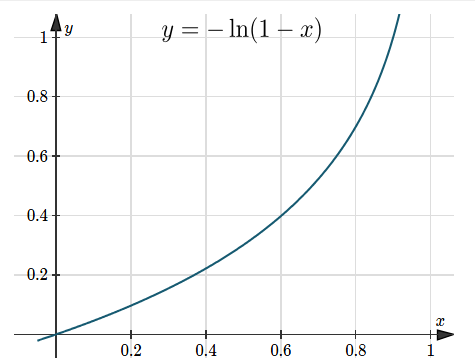
\includegraphics[width=2.8in]
{autoregulons/-log(1-x).png}
\caption{Plot of $y=-\ln(1-x)$.}
\label{fig-minus-log-1-minus-x.png}
\end{figure}

Fig.\ref{fig-c1-ffl-triple}
shows the waveforms for $x(t), y(t), z(t)$
assuming $x(t)$ is either 
a step function rising from 0 at $t=0$,
a step function falling to zero at $t=0$,
or a square impulse rising from 0 at time $t=0$
and falling to 0 a while later.

\subsection{I1-FFL}

\beq
\xymatrix{
\rvx \ar@/_1pc/[drr]|\redoplus\ar[r]|\redoplus
&\bigotimes\ar@/_3pc/[drr]|{\redplus}
& \rvy\ar[d]|{\redminus}\ar[l]|
\redominus
&\rvz\ar[d]|{\redminus}
\\
&
& \dot{y}
&
\dot{z} 
}
\left\{
\begin{array}{l}
\dot{y} =-\alp_\rvy y + \beta_\rvy \indi(x>K_{\rvx\rarrow\rvy}
)
\\
\dot{z} = -\alp_\rvz z + \beta_\rvz \indi(x> K_{\rvx\rarrow\rvz})
{\color{red}\indi(y<K_{\rvy\rarrow\rvz})}
\end{array}
\right.
\eeq


\begin{figure}[h!]
\centering
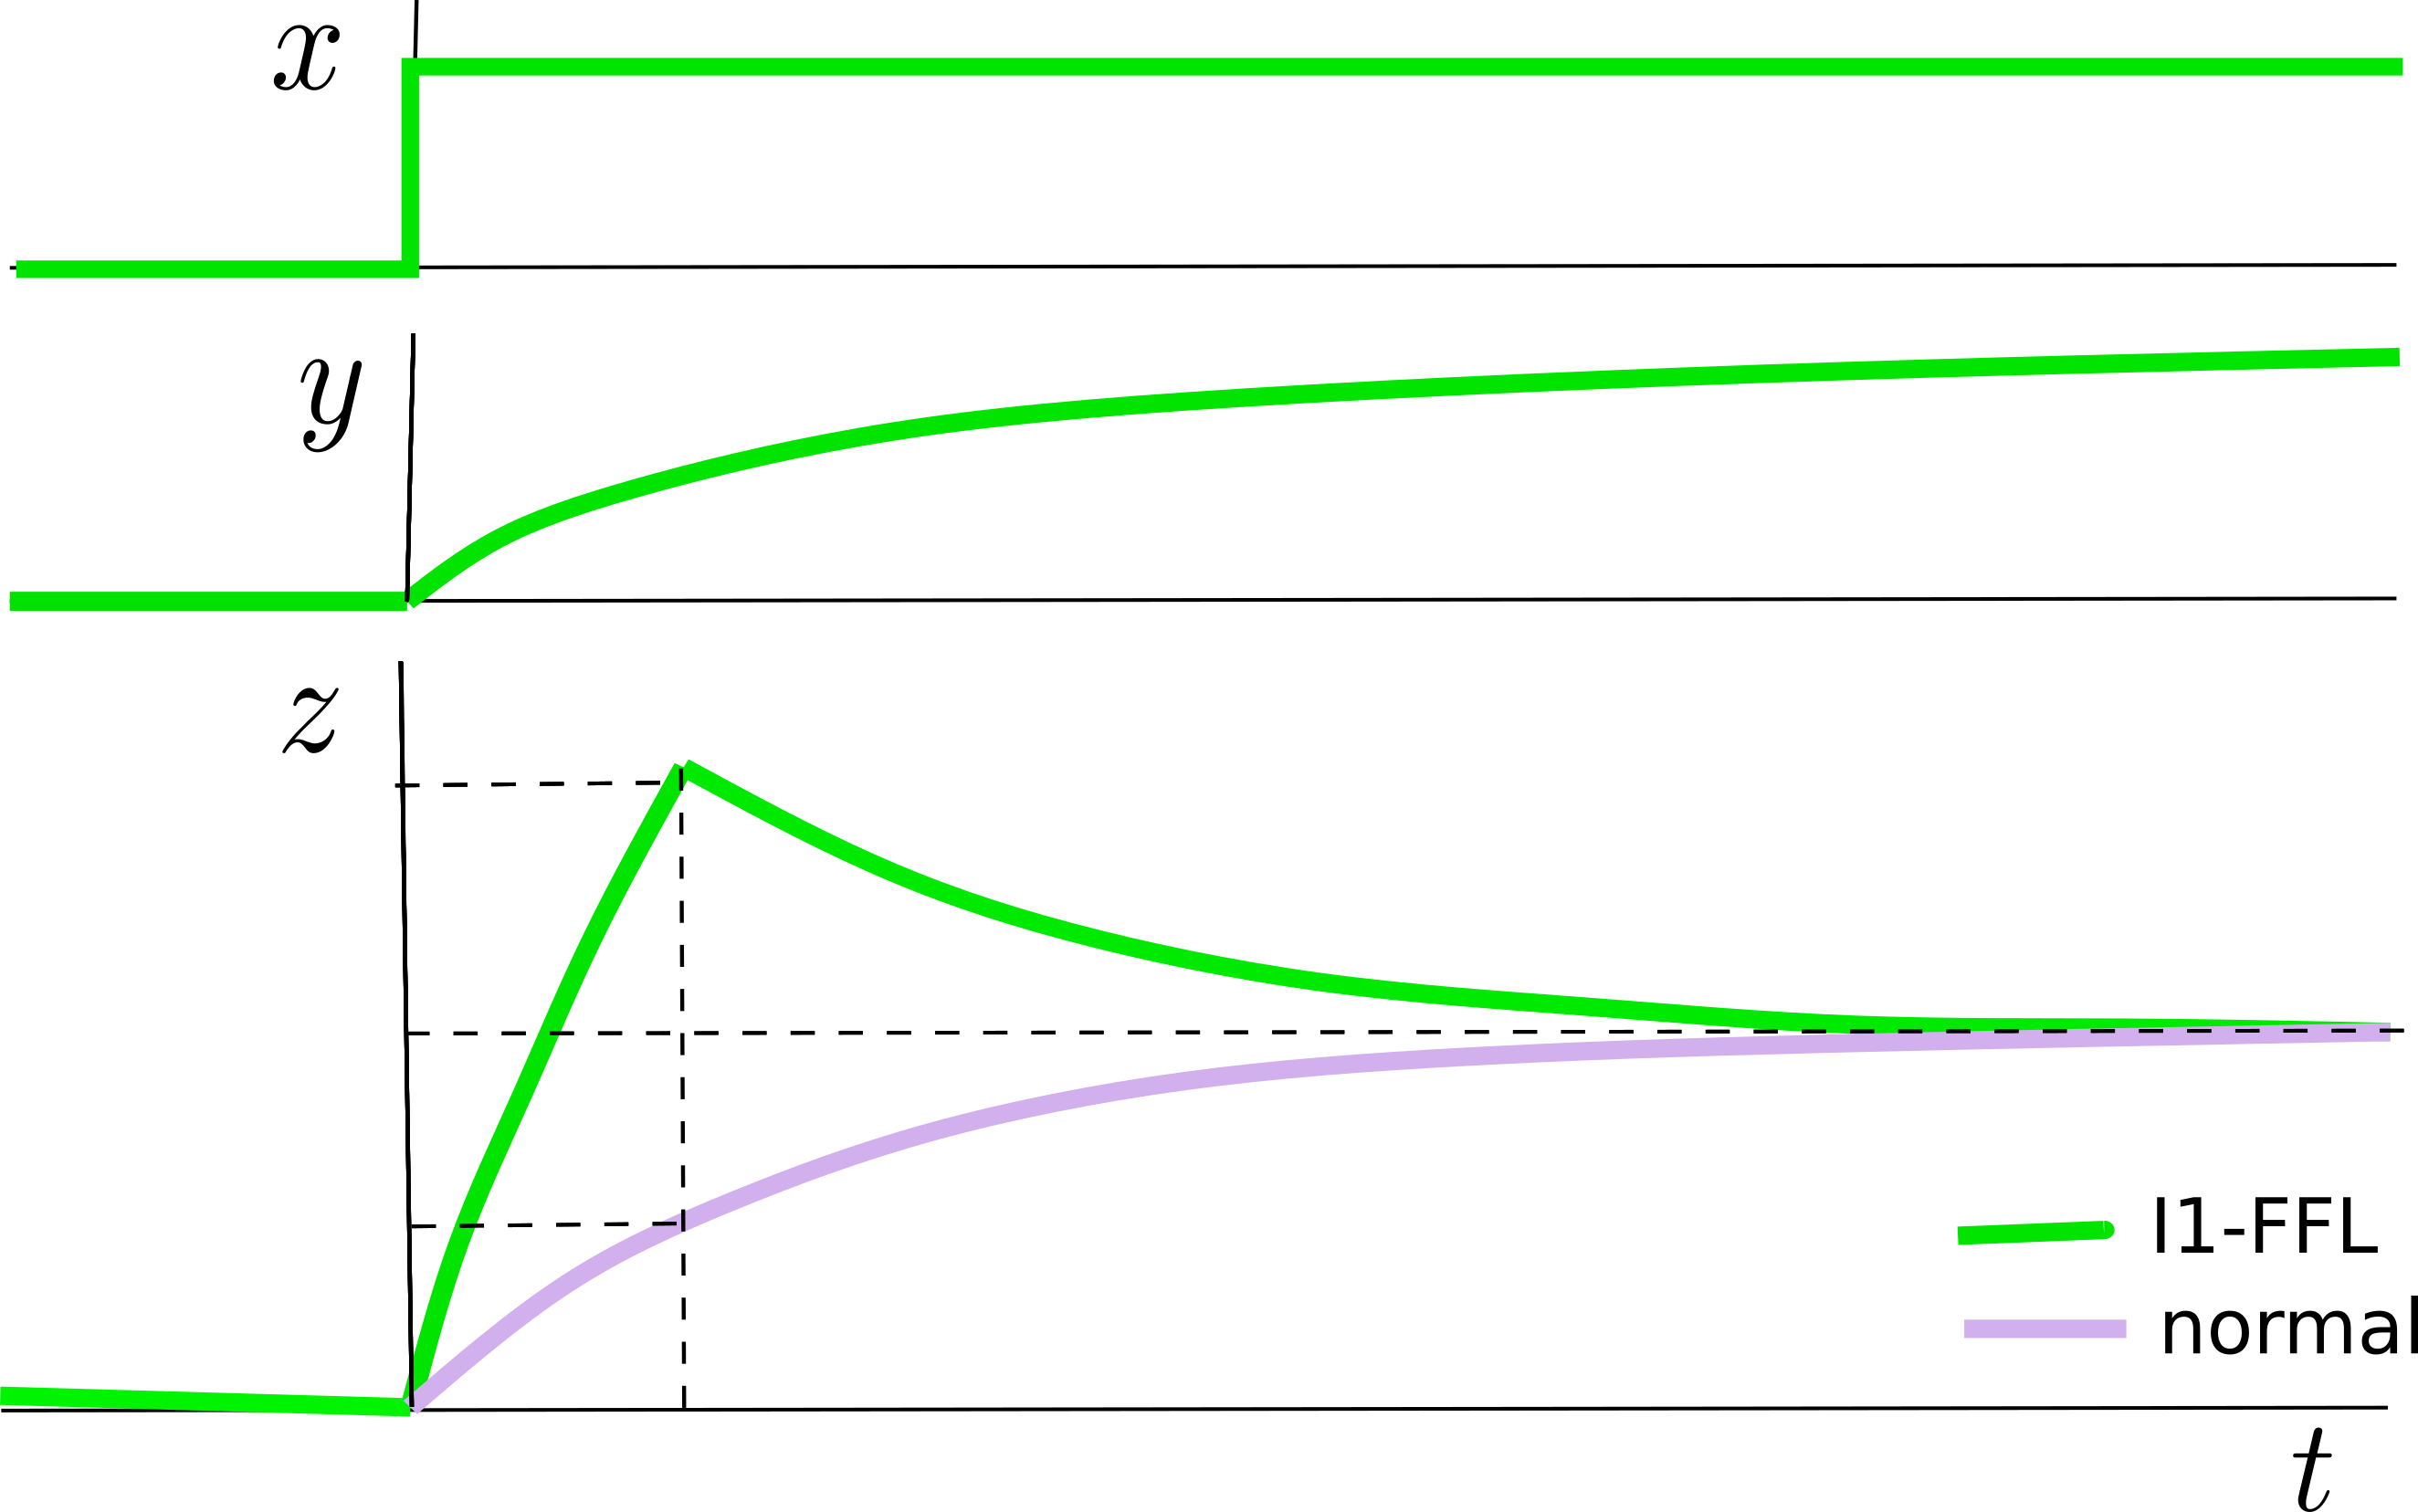
\includegraphics[width=2.8in]
{autoregulons/i1-ffl-green.png}
\caption{For I1-FFL, $x(t), y(t), z(t)$
assuming $x(t)$ step function rising 
from 0 at $t=0$.}
\label{fig-i1-ffl}
\end{figure}

\beq
z=\left\{
\begin{array}{ll}
\frac{\beta_z}{\alp_\rvz}(1- e^{-\alp_\rvz t})
& \text{ for } t<t_{max}
\\
y_{max}e^{-\alp_\rvz (t-t_{max})}
& \text{ for } t> t_{max}
\end{array}
\right.
\eeq
where 

\beq
y_{max}= \frac{\beta_\rvz}{\alp_\rvz}
(1-e^{-\alp_\rvz t_{max}})
\eeq

\subsection{Cascades of multiple autoregulons}

Positive and Negative
cascades of autoregulons.

\beq\begin{array}{ccc}
(a)&
\xymatrix@C =3.5pc{
\Rect{\rvx}\ar[r]|\redplus
&\Rect{\rvy}\ar[r]|\redplus
&\Rect{\rvz}
}
&
\left\{
\begin{array}{l}
\dot{x}= -\alp_1 x
\\
\dot{y}= -\alp_2 y + \gamma_2 x
\\
\dot{z}= -\alp_3 z + \gamma_3 y
\end{array}
\right.
\\
\\
(b)&
\xymatrix@C=3.5pc{
\Rect{\rvx}\ar[r]|\redminus
&\Rect{\rvy}\ar[r]|\redminus
&\Rect{\rvz}
}
&\left\{
\begin{array}{l}
\dot{x}= -\alp_1 x
\\
\dot{y}= -\alp_2 y - \gamma_2 x
\\
\dot{z}= -\alp_3 z - \gamma_3 y
\end{array}
\right.
\end{array}
\eeq


\subsection{Repressilator}
See Ref.\cite{liepe2013maximizing}

Repressilator net

\beq
\xymatrix{
&\ar[r]&\rvm_1\ar[dr]|\redplus
\ar[d]|\redminus
&\rvp_1\ar[d]|\redminus
\ar@/_1pc/[dddlll]|\redominus
\\
\ar[d]&&\dot{\rvm_1}
&\dot{\rvp_1}&\ar[d]
\\
\rvm_2\ar[dr]|\redplus
\ar[d]|\redminus
&\rvp_2\ar[d]|\redminus
\ar[drrr]|\redominus
&&&\rvm_3\ar[dr]|\redplus
\ar[d]|\redminus
&\rvp_3\ar[d]|\redminus
\ar[lllu]|\redominus
\\
\dot{\rvm_2}&\dot{\rvp_2}
&&&\dot{\rvm_3}&\dot{\rvp_3}
}
\left\{
\begin{array}{l}
\dot{m_1} = -m_1 + \frac{\alp}{1+p_3^h}+\alp_0
\\
\dot{m_2} = -m_2 + \frac{\alp}{1+p_1^h}+\alp_0
\\
\dot{m_3} = -m_3 + \frac{\alp}{1+p_2^h}+\alp_0
\\
\dot{p_i} = \beta(m_i-p_i)\quad \text{ for } i=1,2,3
\end{array}
\right.
\eeq

\beq
\dot{y}=-A y
\eeq

\beq
A=
\left[
\begin{array}{ccc}
\alp_1 & 0&\gamma_1
\\
\gamma_2&\alp_2&0
\\
0&-\gamma_3&\alp_3
\end{array}
\right]
\eeq

\beq
y = y_0 e^{-\lam t}
\implies (A-\lam)y=0
\eeq

\beq
\det (A -\lam) = (\alp_1-\lam)(\alp_2-\lam)
(\alp_3 -\lam) - \gamma_1 \gamma_2 \gamma_3
\eeq
For $\alp_1=\alp_2=\alp_3=0$,
get 

\beqa
\lam &=& (-\gamma_1\gamma_2\gamma_3)^{\frac{1}{3}}
\\
&=&
(\gamma_1\gamma_2\gamma_3)^{\frac{1}{3}}
e^{i\frac{1}{3}(-\pi + 2\pi n)}
\eeqa
for $n=0,1,2$


\subsection{Regulated feedback with 3 autoregulons}


Net for Regulated Feedback with 3 autoregulons. All 4 arrows can be either
$\redplus$ or $\redminus$.

\beq
\xymatrix
{\Rect{\rvx}\ar[dr]
\fbackar{rr}{}{}
&&\Rect{\rvy}\ar[dl]
\\
&\Rect{\rvz}
}
\left\{
\begin{array}{l}
\dot{x}= -\alp_1x +ry
\\
\dot{y}= -\alp_2y +sx 
\\
\dot{z}= -\alp_3z + \gamma_1x + 
\gamma_2 y 
\end{array}
\right.
\eeq


\subsection{SIM net}
Single Input Module (SIM) net

SIM net

\beq
\xymatrix@R=4pc{
&\Rect{\rvx}
\ar[dl]|\redoplus_{K_1}
\ar[d]|\redoplus_{K_2}
\ar[dr]|\redoplus^{K_3}
\\
\Rect{\rvz_1}
&\Rect{\rvz_2}
&\Rect{\rvz_3}
}
\left\{
\begin{array}{ll}
\dot{\rvx} =-\alp x +\beta\indi(x< K)
\\
\dot {\rvz_i} =-\alp x_i + \beta_i\indi(x>K_i)
& \text{for $i=1,2,3$}
\end{array}
\right.
\eeq

\begin{figure}[h!]
\centering
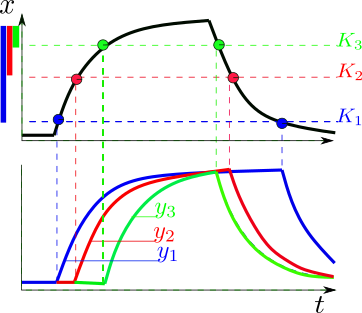
\includegraphics[width=2.8in]
{autoregulons/sim-net.png}
\caption{For SIM net, response  $z_1(t), z_2(t), z_3(t)$ to stimulus $x(t)$.}
\label{fig-sim-net}
\end{figure}


\newpage
\subsection{Flagellum net}

\begin{figure}[h!]
$$
\xymatrix@C=3pc{
&\Rect{\rvx}\ar[d]
\ar[ddl]|\redoplus_{K_1}
\ar[ddr]|\redoplus^{K_2}
\\
&\Rect{\rvy}\ar[dl]|\redoplus^{K'_1}
\ar[dr]|\redoplus_{K'_2}
\\
\Rect{\rvz_1}&
&\Rect{\rvz_2}
}
$$
\caption{Flagellum bnet. Assume $K_1<K_2$ and $K'_1 > K'_2$.}
\label{fig-flagellum}
\end{figure}

\begin{figure}[h!]
\centering
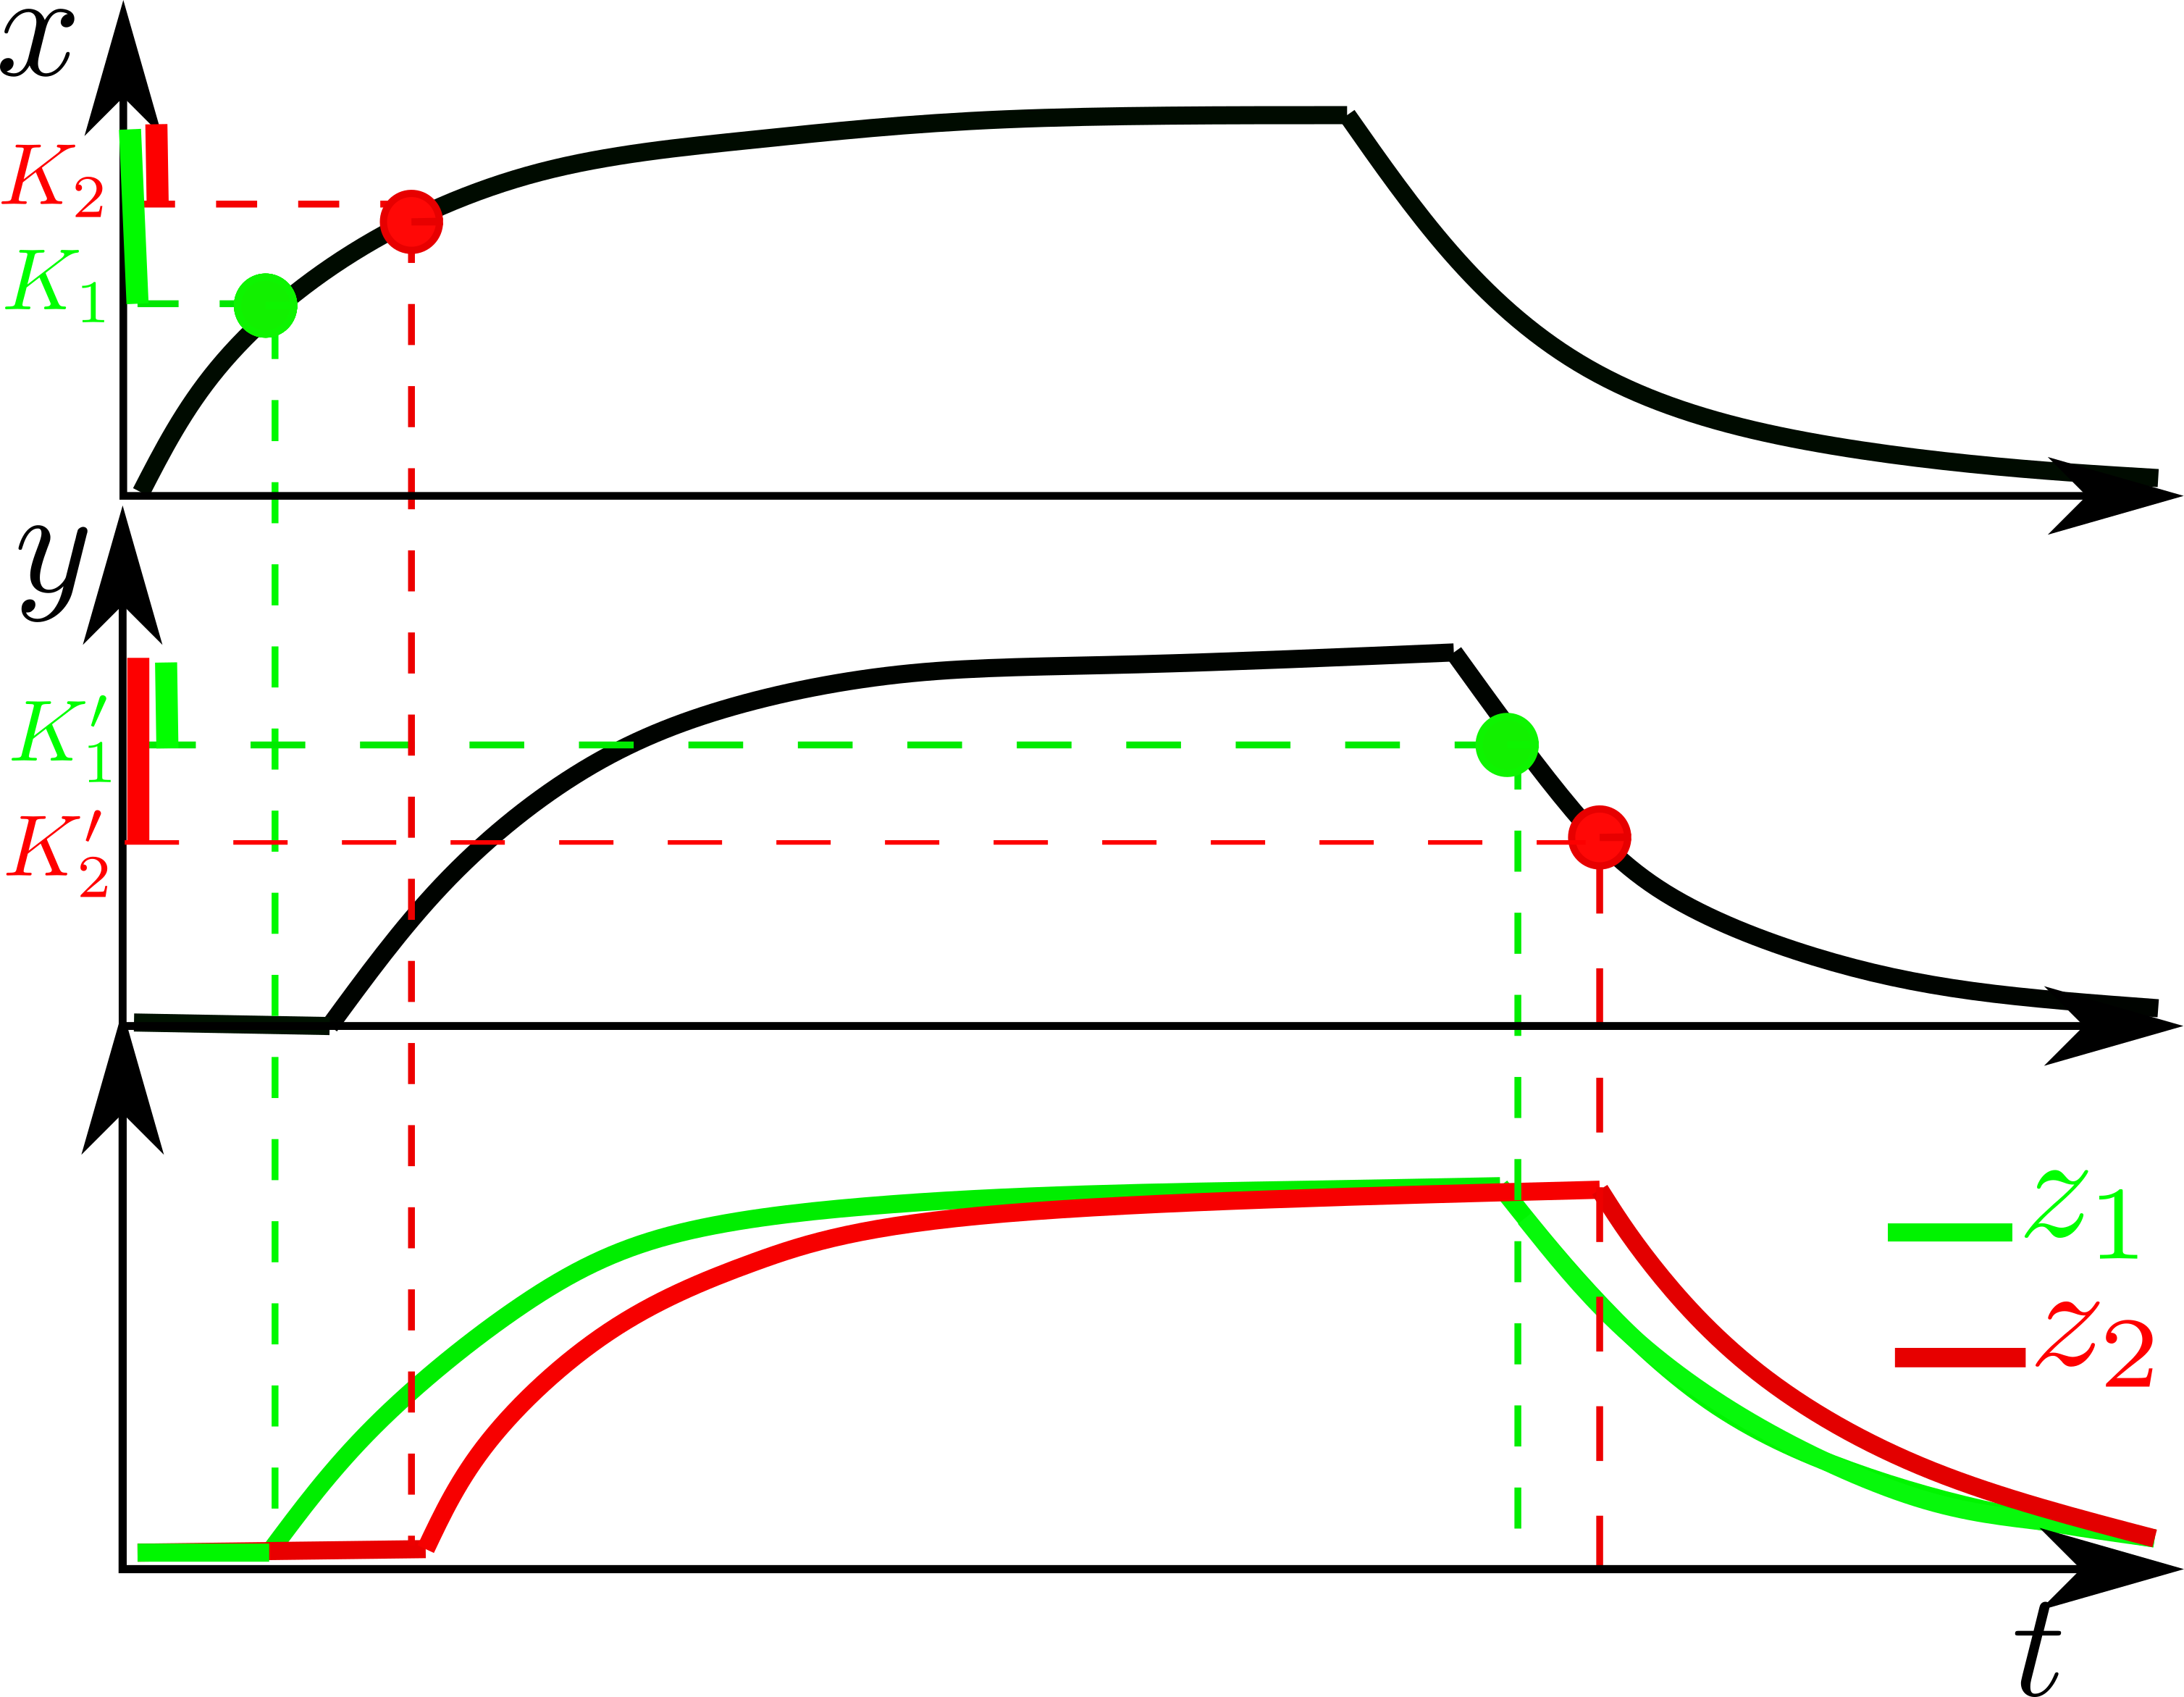
\includegraphics[width=2.8in]
{autoregulons/flagellum.png}
\caption{For Flagellum net, response  $y(t), z_1(t), z_2(t)$ to stimulus $x(t)$.}
\label{fig-flagellum-net}
\end{figure}


\subsection{Bacillus Subtilis Sporation net}

\beq
\xymatrix{
&\Rect{\rvx_1}\ar[ddl]|\redplus
\ar[ddr]|\redplus
\\
&\Rect{\rvy_1}
\ar[dl]|\redminus
\ar[dr]|\redplus
\\
\bigotimes\ar[d]
&&\bigotimes\ar[d]
\\
\Rect{\rvz_1}
&&\Rect{\rvx_2}
\ar[d]|\redplus
\ar[ddl]|\redplus
\ar[ddr]|\redplus
\\
&&\Rect{\rvy_2}\ar[dl]|\redminus
\ar[dr]|\redplus
\\
&\bigotimes\ar[d]
&&\bigotimes\ar[d]
\\
&\Rect{\rvz_2}
&&\Rect{\rvz_3}
}
\eeq
Bacillus Subtilis  Sporation net


\subsection{Frog Egg Cell Cycle net}



Frog egg cell cycle net

\beq
\xymatrix@C=3pc
{\rvx_{u} \ar[rd]\ar@{=>}[d]\ar[r]
& \bigotimes\ar[dl]
& \rvx_p\ar[dr]
\ar[dl]
\ar[l]
\ar@{=>}[d]
& \rvy\ar[dl]\ar@{=>}[d]
\\
\dot{\rvx_{u}}
&\bigotimes\ar[r]
&\dot{\rvx_p}
&\dot{\rvy}}
\left\{
\begin{array}{l}
\dot{x_{u}}= -\PP x_{u} +\PP x_{u} -\PP x_{u}x_p
\\
\dot{x_p}= -\PP x_p  + \PP x_p +
\PP y +\PP x_{u}x_p
\\
\dot{y}= -\PP y +\PP y +\PP x_p
\end{array}
\right.
\eeq

